\documentclass[11pt,a4paper]{article}
\usepackage[utf8]{inputenc}
\usepackage[T1]{fontenc}
\usepackage{lmodern}
\usepackage{geometry}
\usepackage{amsmath,amssymb,amsthm}
\usepackage{booktabs}
\usepackage{longtable}
\usepackage{graphicx}
\usepackage{pdflscape}
\usepackage[hidelinks]{hyperref}
\usepackage{url}

\geometry{margin=2.5cm}
\emergencystretch=3em
\numberwithin{equation}{section}

% Metadata
\title{\bfseries A Finite Computer-Assisted Verification of Robin's Inequality\\
\large via Colossally Abundant Profiles, with Exact Prime-Power Residual Dynamics}
\author{Ing.~Robert~Polak \\ \small robopol@gmail.com \\ \small \url{https://robopol.sk}}
\date{5 August 2026}

% Theorem environments
\newtheorem{theorem}{Theorem}
\newtheorem{proposition}[theorem]{Proposition}
\newtheorem{lemma}[theorem]{Lemma}
\newtheorem{corollary}[theorem]{Corollary}
\theoremstyle{definition}
\newtheorem{definition}[theorem]{Definition}
\newtheorem{remark}[theorem]{Remark}

% Frequently used constants and notation
\newcommand{\Xmin}{3\,299}
\newcommand{\Xdirect}{56\,048\,351}
\newcommand{\Xmax}{164\,967\,000\,000\,000\,000\,000\,000}
\newcommand{\Kcut}{71\,000\,000\,000\,000\,000\,000\,000}
\newcommand{\dd}{\,\mathrm{d}}
\newcommand{\Rinf}{\mathcal R_{\infty}}
\newcommand{\Btwo}{\mathcal B_{2}}
\newcommand{\Cpi}{\mathcal C_{\mathrm{pp}}}
\newcommand{\Ggap}{\mathcal G}
\newcommand{\Bres}{\mathfrak B}
\newcommand{\Bhat}{\widehat{\mathfrak B}}
\newcommand{\sha}[4]{\texttt{#1\allowbreak{}#2\allowbreak{}#3\allowbreak{}#4}}

\begin{document}

\maketitle

\begin{abstract}
We give an unconditional finite, computer-assisted verification of Robin's
inequality
\[
  \sigma(n)<e^\gamma n\log\log n
\]
for every integer
\[
  5041\le n\le 10^{\Kcut}
  =10^{7.1\times10^{22}}.
\]
The proof first certifies the exact logarithmic Robin margin for every
colossally abundant exponent profile whose largest prime factor lies between
\(\Xmin\) and
\[
  \Xmax=1.64967\times10^{23}.
\]
It combines an exhaustive directed-interval enumeration of
\(3\,341\,978\) finite profiles with an analytic prime-power reduction, a
smoothed explicit formula, rigorous finite-height verification of the
Riemann hypothesis, and an absolute estimate for the unverified zero tail.
Robin's convexity proposition between consecutive colossally abundant
numbers then transfers the endpoint result to every integer in the stated
range.

Separately from that finite certificate, we retain the signs discarded by
the absolute high-zero estimate.  We derive an exact recombination of the
integrated prime residual with the deterministic buffer, isolate a continuous
spectral residual \(\Bres(t)\), and prove its prime-power cell equation.  The
one-sided quantity \(2+\gamma-\log(4\pi)-\Bres(t)\) admits a first-crossing
cone whose smooth flow replenishes a scalar reserve and whose prime-power
events withdraw exactly \(\Lambda(q)/\sqrt q\).  Eventual nonnegativity of the
one-sided quantity is RH-equivalent; the cone turns it into a precise
RH-sufficient eventwise target rather than merely a request for a tighter
absolute envelope.  The positivity principle is of known Weil--Suzuki type;
the reformulation developed here is its exact prime-side cell and kick
dynamics.  We further derive an exact signed triangular identity that
reconstructs the post-event slope from an adaptive window of additive size
\(\asymp\sqrt q\log q\).  It isolates a sharp combined prime-side inequality
and a modular Tur\'an-type route.  The latter is RH-conditional and cannot be
used as an unconditional proof step.  A binary64 scan over all
\(5\,762\,859\) prime-power events through \(10^8\) supports the finite
pattern.  An exact hyperbolic prime-side reduction further shows that, for
\(H=\lambda\sqrt q\log q\),
\[
 E_h(q)=\frac{\Delta_H(q)}{2\sqrt q}
 +O_\lambda\!\left(\frac{(\log q)^3}{\sqrt q}\right),
\]
where \(\Delta_H\) is the odd triangular von Mangoldt discrepancy between
the two adjacent half-windows.  A full-population scaling audit finds the
stable bulk normalization \(\sqrt q\,|E_h|/(Q\log q)\), while a classical
Selberg-integral estimate proves unconditional decay of the raw numerator in
measure over continuous dyadic blocks.  Neither averaged decay nor the
finite scan supplies the required uniform estimate at every prime-power
event, and neither universal eventwise target is proved here.

All calculations used in the two finite theorems use deterministic sieves,
exact integer arithmetic, and outward-rounded arbitrary-precision decimal
intervals.  The source and report hashes are recorded.  The conclusion is
finite: it neither proves Robin's inequality for all integers nor proves the
Riemann hypothesis.
\end{abstract}

\section{Introduction and precise scope}

For \(n\ge1\), let
\[
  \sigma(n)=\sum_{d\mid n}d
\]
and let \(\gamma\) be Euler's constant.  Robin proved that the Riemann
hypothesis is equivalent to
\[
  \sigma(n)<e^\gamma n\log\log n
  \qquad(n>5040)
\]
\cite{robin1984}.  This paper does not resolve the infinite quantifier in
Robin's criterion.  Its
first purpose is to isolate and prove a large explicit finite theorem; its
second is to formulate the remaining signed problem as an exact prime-power
dynamical target.

Define the exact logarithmic Robin margin
\begin{equation}\label{eq:G-def}
  \Ggap(n)
  :=
  \gamma+\log\log\log n-\log\frac{\sigma(n)}n.
\end{equation}
For \(n>e^e\), Robin's inequality is equivalent to
\(\Ggap(n)>0\).

An integer \(C\) is \emph{colossally abundant} (CA) if there exists
\(\varepsilon>0\) such that
\[
  \frac{\sigma(m)}{m^{1+\varepsilon}}
  \le
  \frac{\sigma(C)}{C^{1+\varepsilon}}
  \qquad(m\ge1).
\]
At a transition value of \(\varepsilon\), several integers can maximize the
same objective.  Every such tied maximizer is included in the term
\emph{CA profile} below.  We use the classical multiplicative description and
threshold structure of CA numbers due to Alaoglu and Erd\H{o}s
\cite{alaogluerdos1944}.

The two main results are as follows.

\begin{theorem}[Finite CA theorem]\label{thm:finite-ca}
Let \(C\) be any CA profile with exact prime support
\[
  \Xmin\le P(C)\le\Xmax,
\]
where \(P(C)\) is the largest prime factor of \(C\).  Then
\[
  \Ggap(C)>0.
\]
More precisely, with \(x=P(C)\),
\[
  \sqrt{x}\log x\,\Ggap(C)>2\times10^{-7}.
\]
\end{theorem}

\begin{theorem}[Finite all-integer theorem]\label{thm:all-integers}
For every integer \(n\) satisfying
\[
  5041\le n\le10^{\Kcut}
  =10^{7.1\times10^{22}},
\]
one has
\[
  \sigma(n)<e^\gamma n\log\log n.
\]
\end{theorem}

Theorem~\ref{thm:finite-ca} is proved by two overlapping mechanisms.  A direct
all-profile interval computation covers
\[
  \Xmin\le P(C)\le\Xdirect.
\]
An analytic residual certificate, uniform over every CA exponent profile,
covers
\[
  \Xdirect\le P(C)\le\Xmax.
\]
Theorem~\ref{thm:all-integers} is then obtained from a direct base interval,
an exact CA endpoint overlap, the complete intervening CA chain, Robin's
interpolation proposition, and an explicit conversion from prime support to
the size of a CA integer.

After proving these finite statements, Section~\ref{sec:signed-dynamics}
returns to the signed residual before absolute values are taken.  It gives an
exact prime-side dynamical formulation of the post-cutoff obstruction,
including a hyperbolic-to-additive reduction of the signed triangular
discrepancy and an unconditional almost-all continuous-center decay theorem.
The latter is an averaged theorem, not an eventwise prime-power estimate.
None of the exploratory numerical observations in that section is used in
Theorems~\ref{thm:finite-ca} or~\ref{thm:all-integers}.

This finite certificate is logically separate from the RH-strength claims
audited in the corrected status manuscript \cite{polakstatus2026}.  In
particular, the two earlier manuscripts are not altered or silently used as
proofs of the finite numerical assertions made here.

The proofs of the two finite theorems use only the exact identity
\eqref{eq:transformed-margin}, which follows by direct algebra.  They use
neither the MVDC centre \(K(Y,x)\), the reciprocal-prime route, nor any MVDC
estimate.

\begin{remark}[Meaning of computer-assisted]
No random sampling is used.  The finite profile computation exhausts every
support and every transition branch in its domain.  The analytic continuation
uses monotonicity on closed segments and directed interval endpoints.
Nevertheless, the executable certificates are not proof-assistant kernels:
their implementations and documented runtime semantics belong to the trusted
base.
\end{remark}

\section{The exact Robin ledger on full prime support}

Let
\[
  \beta(x)=\prod_{p\le x}\frac{p}{p-1},
  \qquad
  E(x)=\log\beta(x)-\gamma-\log\log x.
\]
For an integer with full support through \(x\),
\[
  n=\prod_{p\le x}p^{a_p},
  \qquad a_p\ge1,
\]
put
\[
  A(n,x)
  =
  -\sum_{p\le x}\log\left(1-p^{-(a_p+1)}\right)
\]
and
\[
  B_{\log}(n,x)
  =
  \log\frac{\log\log n}{\log x}.
\]
The factorization
\[
  \frac{\sigma(n)}n
  =
  \beta(x)\prod_{p\le x}\left(1-p^{-(a_p+1)}\right)
\]
gives the following exact identity.

\begin{lemma}[Exact Robin gate]\label{lem:exact-gate}
For every full-support \(n\) as above,
\begin{equation}\label{eq:exact-gate}
  \Ggap(n)=A(n,x)+B_{\log}(n,x)-E(x).
\end{equation}
Consequently Robin's inequality is equivalent to the positivity of the
right-hand side.
\end{lemma}

\begin{proof}
Taking logarithms in the product for \(\sigma(n)/n\) gives
\[
  \log\frac{\sigma(n)}n
  =
  \gamma+\log\log x+E(x)-A(n,x).
\]
On the other hand,
\[
  \gamma+\log\log\log n
  =
  \gamma+\log\log x+B_{\log}(n,x).
\]
Subtracting proves \eqref{eq:exact-gate}.
\end{proof}

For later use, define
\[
  \theta(x)=\sum_{p\le x}\log p,
  \qquad
  \psi(x)=\sum_{p^m\le x}\log p,
\]
\[
  H(n,x)=\log n-\theta(x),
  \qquad
  z(n,x)=\frac{\log n-x}{x},
  \qquad
  L=\log x.
\]
Then
\[
  \log\log n=L+\log(1+z),
\]
so the nonlinear bridge remainder is
\begin{equation}\label{eq:B2-def}
  \Btwo(n,x)
  =
  \log\left(1+\frac{\log(1+z(n,x))}{L}\right)
  -\frac{z(n,x)}L.
\end{equation}

\section{Exact prime-power reduction}

Put
\[
  F(t)=\frac1{t\log t},
  \qquad
  \omega(t)=-F'(t)
  =\frac{\log t+1}{t^2\log^2t},
\]
and define the smoothed prime-distribution residual
\begin{equation}\label{eq:Rinf-def}
  \Rinf(x)=\int_x^\infty(\psi(t)-t)\omega(t)\dd t.
\end{equation}
Its convergence is justified in Section~\ref{sec:explicit-formula}, where the
integrated zero series is shown to be absolutely convergent.

Let
\[
  \mathcal H_\Lambda(x)
  =\sum_{2\le n\le x}\frac{\Lambda(n)}{n\log n}
  =\sum_{p^m\le x}\frac1{mp^m}.
\]

\begin{lemma}[Finite prime-side form of the residual]
\label{lem:Rinf-prime-side}
For every real \(x>1\), with either consistent one-sided convention at a
prime-power endpoint,
\begin{equation}\label{eq:Rinf-prime-side}
  \boxed{
  \Rinf(x)
  =\frac{\psi(x)-x}{x\log x}
  +\gamma+\log\log x-\mathcal H_\Lambda(x).
  }
\end{equation}
The right-hand side is continuous at every prime power.
\end{lemma}

\begin{proof}
Stieltjes integration up to \(Y>x\) gives
\begin{align*}
  \int_x^Y(\psi(t)-t)\omega(t)\dd t
  ={}&\frac{\psi(x)-x}{x\log x}
  -\frac{\psi(Y)-Y}{Y\log Y}\\
  &+\sum_{x<n\le Y}\frac{\Lambda(n)}{n\log n}
  -\log\log Y+\log\log x.
\end{align*}
The PNT removes the boundary term, while
  \(\mathcal H_\Lambda(Y)=\log\log Y+\gamma+o(1)\).  Letting \(Y\) tend to
infinity proves \eqref{eq:Rinf-prime-side}.  At \(x=p^m\), the endpoint term
jumps by \(1/(mp^m)\), exactly as does \(\mathcal H_\Lambda\).
\end{proof}

Also define
\begin{equation}\label{eq:Rcore-def}
  R_{\mathrm{core}}(n,x)
  =
  \frac{H(n,x)}{x\log x}
  -\sum_{p\le x}\log\left(1-p^{-(a_p+1)}\right).
\end{equation}

\subsection{The finite prime-power correction}

Let
\[
  \mathcal P_\infty(x)
  =
  \int_x^\infty(\psi(t)-\theta(t))\omega(t)\dd t
\]
and
\[
  \mathcal T_2(x,\infty)
  =
  \sum_{p>x}\sum_{m\ge2}\frac1{mp^m}.
\]
Since \(\psi-\theta\ge0\), Tonelli's theorem and
\[
  \log p\,F(p^m)=\frac1{mp^m}
\]
give
\[
  \mathcal P_\infty(x)
  =
  \frac{\psi(x)-\theta(x)}{x\log x}
  +
  \sum_{\substack{p,m\ge2\\p^m>x}}\frac1{mp^m}.
\]
The bases \(p>x\) cancel on subtracting \(\mathcal T_2\).  Thus
\begin{equation}\label{eq:Cpp-def}
  \Cpi(x)
  :=
  \mathcal P_\infty(x)-\mathcal T_2(x,\infty)
  =
  \frac{\psi(x)-\theta(x)}{x\log x}
  +
  \sum_{\substack{p\le x,\ m\ge2\\p^m>x}}\frac1{mp^m}.
\end{equation}
This is a finite prime-power quantity.

Let
\[
  W(x)
  =
  E(x)-\frac{\theta(x)-x}{x\log x}.
\]
Partial summation of the first-order prime sum, followed by the convergent
Euler-product tail, yields
\[
  W(x)
  =
  \int_x^\infty(t-\theta(t))\omega(t)\dd t
  -\mathcal T_2(x,\infty).
\]
Since
\[
  \mathcal P_\infty(x)-\Rinf(x)
  =
  \int_x^\infty(t-\theta(t))\omega(t)\dd t,
\]
we obtain the exact relation
\begin{equation}\label{eq:W-C-R}
  W(x)=\Cpi(x)-\Rinf(x).
\end{equation}

\begin{proposition}[Exact Robin-gap identity]\label{prop:transformed-margin}
For every full-support exponent vector,
\begin{equation}\label{eq:transformed-margin}
  \boxed{
  \Ggap(n)
  =
  \Rinf(x)+\Btwo(n,x)
  +R_{\mathrm{core}}(n,x)-\Cpi(x).
  }
\end{equation}
\end{proposition}

\begin{proof}
By \eqref{eq:B2-def},
\[
  B_{\log}(n,x)
  =
  \frac{z(n,x)}L+\Btwo(n,x).
\]
Moreover,
\[
  z(n,x)
  =
  \frac{\theta(x)-x+H(n,x)}x.
\]
Substituting these identities and
\[
  E(x)=\frac{\theta(x)-x}{xL}+W(x)
\]
into Lemma~\ref{lem:exact-gate} cancels the endpoint term
\((\theta(x)-x)/(xL)\).  Equation \eqref{eq:W-C-R} then gives
\eqref{eq:transformed-margin}.
\end{proof}

\subsection{A positive profile-independent core}

For \(p\le x\), let
\[
  k_p(x)=\max\{k\ge1:p^k\le x\},
\]
\[
  c_{p,x}=\frac{\log p}{x\log x},
  \qquad
  d_{p,a}=-\log\left(1-p^{-(a+1)}\right),
\]
and
\[
  \Phi_{p,x}(a)=(a-1)c_{p,x}+d_{p,a}.
\]
Then
\[
  R_{\mathrm{core}}(n,x)=\sum_{p\le x}\Phi_{p,x}(a_p).
\]
Also put
\[
  Q_{p,k}
  =
  \sum_{m=k+1}^{\infty}\frac1{mp^m}.
\]
Equation \eqref{eq:Cpp-def} becomes
\begin{equation}\label{eq:Cpp-prime-sum}
  \Cpi(x)
  =
  \sum_{p\le x}
  \left((k_p-1)c_{p,x}+Q_{p,k_p}\right).
\end{equation}

\begin{lemma}[Strict prime-by-prime domination]\label{lem:prime-domination}
For every real \(x\ge2\), every prime \(p\le x\), and every integer \(a\ge1\),
\[
  \Phi_{p,x}(a)>
  (k_p-1)c_{p,x}+Q_{p,k_p}.
\]
\end{lemma}

\begin{proof}
Write
\[
  \delta_{p,a}
  =
  d_{p,a}-d_{p,a+1}
  =
  \log\left(
  1+\frac1{p+p^2+\cdots+p^{a+1}}
  \right).
\]
The sequence \(\delta_{p,a}\) is strictly decreasing and
\[
  \Phi_{p,x}(a+1)-\Phi_{p,x}(a)
  =
  c_{p,x}-\delta_{p,a}.
\]
Let \(k=k_p\).  If \(a<k\), then \(k\ge2\), and
\[
  \delta_{p,k-1}>
  \frac1{1+p+\cdots+p^k}
  \ge\frac1{kp^k}
  \ge c_{p,x}.
\]
Here \(1+p+\cdots+p^k<2p^k\le kp^k\), while
\(x\log x\ge kp^k\log p\).
Thus \(\Phi_{p,x}\) decreases strictly through index \(k\), and
\(\Phi_{p,x}(a)>\Phi_{p,x}(k)\).

For \(a\ge k\), set
\[
  u=\frac1{(k+1)p^{k+1}}.
\]
Since \(p^k\le x<p^{k+1}\),
\[
  c_{p,x}>u,
  \qquad
  Q_{p,k}\le\frac{u}{1-1/p}.
\]
If \(a=k\), then
\[
  d_{p,k}>p^{-(k+1)}
  =(k+1)u\ge\frac{u}{1-1/p}.
\]
If \(a=k+1\), then
\[
  c_{p,x}+d_{p,k+1}
  >
  u+\frac1{p^{k+2}}
  =
  u\left(1+\frac{k+1}{p}\right)
  \ge\frac{u}{1-1/p}.
\]
If \(a\ge k+2\), then
\[
  (a-k)c_{p,x}>2u\ge\frac{u}{1-1/p}.
\]
These cases prove the claim.
\end{proof}

Define the optimal full-support core and its finite buffer by
\begin{equation}\label{eq:Dstar-def}
  R_*(x)=\sum_{p\le x}\min_{a\ge1}\Phi_{p,x}(a),
  \qquad
  D_*(x)=R_*(x)-\Cpi(x).
\end{equation}

\begin{corollary}\label{cor:Dstar-positive}
For every \(x\ge2\),
\[
  R_{\mathrm{core}}(n,x)-\Cpi(x)\ge D_*(x)>0.
\]
Consequently it is sufficient to prove
\begin{equation}\label{eq:residual-target}
  \Rinf(x)+\Btwo(n,x)>-D_*(x).
\end{equation}
\end{corollary}

The minimizing exponent is characterized by
\[
  a_p^*(x)
  =
  \min\left\{
  a\ge1:
  \delta_{p,a}\le\frac{\log p}{x\log x}
  \right\}.
\]
If equality occurs, the adjacent exponents have the same value of
\(\Phi_{p,x}\); hence \(D_*\) is tie-safe.  Notice that this
full-support optimizer is not the CA-family activation rule
\(\tau_s(p)>\tau_1(x)\).

\section{Certified lower bounds for the deterministic buffer}

\subsection{Complete finite sweep}

\begin{proposition}[Finite \(D_*\) certificate]\label{prop:Dstar-finite}
At every one of the \(3\,340\,551\) prime supports
\[
  \Xmin\le x\le\Xdirect,
\]
the directed interval certificate proves
\[
  \sqrt{x}\log x\,D_*(x)>0.7825.
\]
The certified global minimum lower endpoint is
\[
  0.7825999188377564057191055633151903716957
\]
at \(x=\Xdirect\).
\end{proposition}

The verifier uses a deterministic odd-only sieve, exact integer prime-power
events, outward-rounded logarithms and square roots, and rigorous alternating
series bounds above a fixed exact-log cutoff.  It reports no failed or
inconclusive support.  Direct reconstructions at
\(3299,5297,5303,10007\) overlap the streamed intervals; the pair
\(5297,5303\) straddles a change between the CA-only and full-support
activation conventions.

\subsection{Analytic continuation beyond the sieve}

Put
\[
  y=\sqrt{2x},\qquad
  L=\log x,\qquad
  \ell=\log y=\frac{L+\log2}{2}.
\]
For \(y<p\le x\), one has \(p^2>x\), and the exact optimizer is
\(a_p^*(x)=1\).  Indeed,
\[
  \frac{\delta_{p,1}}{\log p}
  =
  \frac1{\log p}\log\left(1+\frac1{p+p^2}\right)
  <
  \frac1{p^2\log p}
  <
  \frac1{x\log x},
\]
where the last inequality follows from \(p^2>2x\) and
\(\log p>\tfrac12\log x\).  The characterization preceding
Proposition~\ref{prop:Dstar-finite} now gives the claim.  The corresponding
contribution to \(D_*(x)\) is
\[
  d_{p,1}-Q_{p,1}
  =
  \frac1p-\log\left(1+\frac1p\right)
  >
  \left(\frac12-\frac1{3y}\right)\frac1{p^2}.
\]
All omitted prime contributions are positive.

Use Dusart's explicit estimate
\begin{equation}\label{eq:dusart-theta}
  |\theta(t)-t|<\frac{3.965t}{\log^2t}
  \qquad(t\ge2)
\end{equation}
\cite{dusarttheta1999}.  Partial summation over \(y<p\le x\) gives the
following closed lower expression.  Put
\[
  \epsilon=\frac{3.965}{\ell^2},
  \qquad
  q(x)=1-\sqrt{\frac2x},
\]
\[
  A(L)=\frac{L}{\sqrt2\,\ell},
  \qquad
  \underline J(L)
  =
  \frac{L}{\sqrt2}
  \left(\frac{q(x)}\ell-\frac1{\ell^2}\right),
\]
\[
  \underline S(L)
  =
  (1-\epsilon)\underline J(L)
  -2\epsilon A(L)-\frac1{\sqrt x},
\]
and
\[
  D_{\mathrm{lb}}(x)
  =
  \left(\frac12-\frac1{3\sqrt{2x}}\right)\underline S(L).
\]

\begin{proposition}[Analytic \(D_*\) continuation]\label{prop:Dstar-analytic}
For every real \(x\ge\Xdirect\),
\[
  \sqrt{x}\log x\,D_*(x)>D_{\mathrm{lb}}(x)>0.5.
\]
Moreover \(D_{\mathrm{lb}}\) is increasing,
\[
  D_{\mathrm{lb}}(\Xdirect)
  >
  0.516114369552624825734994861539,
\]
and
\[
  D_{\mathrm{lb}}(\Xmax)
  >
  0.661088880265812593800990356530.
\]
\end{proposition}

\begin{proof}
Put
\[
  S_2(y,x)=\sum_{y<p\le x}\frac1{p^2}.
\]
Partial summation gives
\[
\begin{aligned}
  S_2(y,x)
  ={}&
  \frac{\theta(x)}{x^2L}
  -\frac{\theta(y)}{y^2\ell}\\
  &+
  \int_y^x\theta(t)
  \left(\frac2{t^3\log t}+\frac1{t^3\log^2t}\right)\dd t.
\end{aligned}
\]
For \(t\in[y,x]\), equation~\eqref{eq:dusart-theta} implies
\((1-\epsilon)t<\theta(t)<(1+\epsilon)t\).  Dropping the nonnegative
endpoint at \(x\), using the upper estimate at the negative \(y\)-endpoint,
and using the lower estimate in the integral yields
\[
  S_2(y,x)
  >
  -\frac{1+\epsilon}{y\ell}
  +(1-\epsilon)
  \left(\frac1{y\ell}-\frac1{xL}+J(y,x)\right),
\]
where
\[
  J(y,x)=\int_y^x\frac{\dd t}{t^2\log t}.
\]
Writing \(r=x/y=\sqrt{x/2}\), substituting \(t=yu\), and using
\[
  \frac1{\ell+\log u}
  \ge
  \frac1\ell-\frac{\log u}{\ell^2}
  \qquad(u\ge1)
\]
gives
\[
  J(y,x)
  >
  \frac1y\left(\frac{1-1/r}{\ell}-\frac1{\ell^2}\right).
\]
Since \(1-1/r=q(x)\), multiplication by \(\sqrt{x}L\) gives
\[
  \sqrt{x}L
  S_2(y,x)
  >
  \underline S(L).
\]
Here replacing \(-(1-\epsilon)/\sqrt{x}\) by \(-1/\sqrt{x}\) only weakens
the lower bound.  The prefactor \(1/2-1/(3\sqrt{2x})\) comes from the
alternating logarithm series.  For monotonicity, \(\epsilon\) decreases;
\(q\), \(L/\ell\), and \(\underline J\) increase;
\(\epsilon A=3.965L/(\sqrt2\,\ell^3)\) decreases because its derivative
has the sign of \(\log2-2L\); and both
\(-x^{-1/2}\) and \(1/2-1/(3\sqrt{2x})\) increase.  The factors
\(1-\epsilon\), \(\underline J\), and the resulting
\(\underline S\) are positive at \(\Xdirect\).  Hence
\(\underline S\) and \(D_{\mathrm{lb}}\) are positive and increasing.
The endpoint evaluations are directed intervals.  The \(60\)- and
\(80\)-digit enclosures are nested.
\end{proof}

\section{Uniform control of the signed residual}

\subsection{Tie-safe CA layer bounds}

For \(s\ge1\), define the CA transition threshold
\[
  \tau_s(p)
  =
  \frac1{\log p}
  \log\frac{1-p^{-(s+1)}}{1-p^{-s}}.
\]
If \(x\) is the exact support and \(q\) is the next prime, the CA parameter
satisfies
\[
  \tau_1(q)\le\varepsilon\le\tau_1(x).
\]
If \(a_p\ge s\ge2\), then \(\varepsilon\le\tau_s(p)\).  Since
\[
  \tau_1(q)>\frac1{(q+1)\log q},
  \qquad
  \tau_s(p)<\frac1{p^s\log p},
\]
one has \(p^s\log p<(q+1)\log q\).  If \(p<q^{1/s}\), the desired
bound is immediate.  Otherwise \(\log q/\log p\le s\), and the same
inequality again gives \(p^s<s(q+1)\).  Thus one obtains the strict,
tie-safe implication
\begin{equation}\label{eq:layer-cutoff}
  a_p\ge s
  \quad\Longrightarrow\quad
  p<(s(q+1))^{1/s}.
\end{equation}
Hence
\[
  H(n,x)
  =
  \sum_{s\ge2}\sum_{a_p\ge s}\log p
  \le
  \sum_{\substack{s\ge2\\(s(q+1))^{1/s}>2}}
  \theta\left((s(q+1))^{1/s}\right).
\]

Dusart's short-prime theorem \cite{dusartprime1999} gives, for \(x\ge3275\),
\[
  q\le x\left(1+\frac1{2\log^2x}\right).
\]
Together with Rosser--Schoenfeld's global estimate
\(\theta(t)<1.01624t\) \cite{rosserschoenfeld1962}, the decreasing
layer majorant gives
\begin{equation}\label{eq:H-upper-large}
  H(n,x)<2.035\sqrt{x}
  \qquad(x\ge\Xdirect)
\end{equation}
through the range used here.  On the lower interval an event-by-event
directed analysis gives
\begin{equation}\label{eq:H-upper-small}
  H(n,x)<2.634\sqrt{x}
  \qquad(\Xmin\le x\le\Xdirect).
\end{equation}
The latter checks the left endpoint and the right limits of the fifteen layer
activation events \(s=16,\ldots,30\); between events the normalized
majorant decreases.

The largest layer cutoff at \(x=\Xmax\) is
\[
  <5.7445\times10^{11}<10^{19}.
\]
Thus B\"uthe's finite theorem \cite{buthe2018} can alternatively be used at
every layer cutoff, where it supplies \(\theta(u)<u\).

\subsection{The nonlinear bridge}

B\"uthe's partial-RH estimate \cite{buthe2016} states that, for \(x\ge5000\),
\begin{equation}\label{eq:buthe-partial}
  |\theta(x)-x|
  \le
  \frac{\sqrt{x}\log x(\log x-2)}{8\pi},
\end{equation}
provided RH has been verified through height \(T\) and
\[
  4.92\sqrt{\frac{x}{\log x}}\le T.
\]
At \(x=\Xmax\), the required height is less than
\[
  273\,305\,915\,796<3\times10^{12}.
\]
Platt and Trudgian rigorously verified RH through
\(3\times10^{12}\) \cite{platttrudgian2021}; hence
\eqref{eq:buthe-partial} holds throughout the upper range.

Combining \eqref{eq:H-upper-large} with \eqref{eq:buthe-partial} gives
\[
  |z(n,x)|
  <
  \delta(L)
  :=
  \left(\frac{L(L-2)}{8\pi}+2.035\right)e^{-L/2}.
\]
The directed endpoint and derivative checks give
\(0<\delta(L)<0.001774<1\) throughout the upper range.
For
\[
  b_L(z)
  =
  \log\left(1+\frac{\log(1+z)}L\right)-\frac zL,
\]
one has \(b_L(0)=b_L'(0)=0\) and
\[
  b_L''(z)
  =
  -\frac{A+1}{(1+z)^2A^2},
  \qquad
  A=L+\log(1+z).
\]
Taylor's theorem at \(z=0\), evaluated at the worst lower endpoint
\(-\delta(L)\), gives a directed lower bound for \(\Btwo\).  Its normalized
upper loss is the explicit function
\begin{equation}\label{eq:CB2-def}
  C_{B_2}(x)
  =
  \frac{\sqrt{x}L\,\delta(L)^2}{2}
  \frac{A_-(L)+1}{(1-\delta(L))^2A_-(L)^2},
  \qquad
  A_-(L)=L+\log(1-\delta(L)),
\end{equation}
so that
\[
  -\sqrt{x}L\,\Btwo(n,x)\le C_{B_2}(x).
\]
This function decreases over the upper range.  At \(x=\Xmax\),
\begin{equation}\label{eq:B2-endpoint}
  -\sqrt{x}L\,\Btwo(n,x)
  <
  1.5589734604839492\times10^{-8}.
\end{equation}

\subsection{Integrated explicit formula}\label{sec:explicit-formula}

Let \(\rho=\beta+i\gamma_\rho\) run over nontrivial zeros of
\(\zeta(s)\), with multiplicity.  Starting from the standard symmetric
truncation of the von Mangoldt explicit formula
\cite[Ch.~17]{titchmarsh1986}, insert a compact upper cutoff and integrate the
finite zero sum against \(\omega\).  After the substitution \(t=e^u\), put
\[
  h(u)=\frac{u+1}{u^2},
  \qquad
  J_\rho(L)
  =
  \int_L^\infty e^{-(1-\rho)u}h(u)\dd u.
\]
For \(\Re z>0\), write
\[
  E_1(z)=\int_1^\infty\frac{e^{-zu}}u\dd u.
\]
One direct integration gives the exact closed form
\begin{equation}\label{eq:Jrho-E1}
  \boxed{
  J_\rho(L)
  =\frac{e^{-(1-\rho)L}}L
  +\rho E_1((1-\rho)L).
  }
\end{equation}
The half-weight convention for \(\psi\) at a jump is immaterial here, because
changing values at the prime-power endpoints does not change the integral.
Passing first through symmetric zero truncations and then through compact
upper cutoffs gives
\begin{equation}\label{eq:integrated-explicit}
  \Rinf(x)
  =
  -\sum_\rho\frac{J_\rho(L)}{\rho}
  -\frac{\log(2\pi)}{xL}
  -\frac12\int_x^\infty
  \log(1-t^{-2})\omega(t)\dd t.
\end{equation}
The last term is positive and may be discarded in a lower bound.

The limiting passage is not justified merely by writing a formal termwise
integral.  Two integrations by parts below give
\[
  \left|\frac{J_\rho(L)}\rho\right|
  =O_L(\gamma_\rho^{-2}).
\]
The zero count \(N(T)=O(T\log T)\) then makes the integrated zero series
absolutely convergent, completing the cutoff argument.

The exact smoothing performed by the integral is visible after multiplying
the zero part by its natural Robin scale.  Define
\[
  A_\rho(L)
  =\frac1\rho
  +Le^{(1-\rho)L}E_1((1-\rho)L).
\]
Then
\begin{equation}\label{eq:normalized-zero-kernel}
  e^{L/2}L\left(-\sum_\rho\frac{J_\rho(L)}\rho\right)
  =-\sum_\rho e^{(\rho-1/2)L}A_\rho(L).
\end{equation}
The identity
\[
  e^zE_1(z)=\int_0^\infty\frac{e^{-v}}{z+v}\dd v
\]
and a two-term geometric expansion give the rigorous remainder formula
\begin{equation}\label{eq:Arho-expansion}
  \boxed{
  A_\rho(L)
  =\frac1{\rho(1-\rho)}
  -\frac1{(1-\rho)^2L}+R_{\rho,2}(L),
  \qquad
  |R_{\rho,2}(L)|
  \le\frac2{|1-\rho|^3L^2}.
  }
\end{equation}
Thus the endpoint Chebyshev error and the logarithmically weighted Mangoldt
error cancel their separate \(1/\gamma_\rho\) coefficients and leave an
absolutely summable \(1/\gamma_\rho^2\) kernel.  They do not cancel the factor
\(e^{(\beta-1/2)L}\).  A hypothetical zero with \(\beta>1/2\) therefore
remains an exponentially growing normalized mode.  This distinction is the
reason that sharper absolute estimates can extend the finite certificate but
cannot by themselves settle the infinite problem.

\subsection{Verified low zeros}

Let \(T=3\times10^{12}\).  By the Platt--Trudgian theorem cited above, every
zero with \(|\gamma_\rho|\le T\) has
\(\rho=1/2+i\gamma_\rho\).  For such a zero, one integration by parts yields
\[
  |J_\rho(L)|
  \le
  \frac{x^{-1/2}}{|1-\rho|}
  \left(
  h(L)+\frac{2(L+2)}{L^3}
  \right).
\]
The exact identity
\[
  \sum_\rho\frac1{\rho(1-\rho)}
  =
  2+\gamma-\log(4\pi)
\]
bounds the verified subset.  Omitted zero pairs have positive real
contribution to this identity because
\[
  \operatorname{Re}\bigl(\rho(1-\rho)\bigr)
  =
  \beta(1-\beta)+\gamma_\rho^2>0.
\]
Consequently the normalized low-zero loss, including the
\(\log(2\pi)\) term, is at most
\begin{equation}\label{eq:low-zero-loss}
  C_{\mathrm{low}}(x)
  =
  \bigl(2+\gamma-\log(4\pi)\bigr)
  \left(1+\frac3L+\frac4{L^2}\right)
  +\frac{\log(2\pi)}{\sqrt{x}}.
\end{equation}
This decreases with \(x\).

\subsection{Unverified high zeros}

Twice integrating \(J_\rho\) by parts gives
\[
  J_\rho(L)
  =
  e^{-(1-\rho)L}
  \left(
  \frac{h(L)}{1-\rho}
  +\frac{h'(L)}{(1-\rho)^2}
  \right)
  +
  \frac1{(1-\rho)^2}
  \int_L^\infty e^{-(1-\rho)u}h''(u)\dd u.
\]
Here
\[
  h'(u)=-\frac1{u^2}-\frac2{u^3},
  \qquad
  h''(u)=\frac2{u^3}+\frac6{u^4}>0.
\]
It follows that
\begin{equation}\label{eq:per-zero-high}
  \left|\frac{J_\rho(L)}{\rho}\right|
  \le
  x^{\beta-1}
  \left(
  \frac{h(L)}{\gamma_\rho^2}
  +\frac{2[-h'(L)]}{|\gamma_\rho|^3}
  \right).
\end{equation}

For every positive ordinate, the functional equation gives the
multiplicity-preserving involution
\[
  \beta+i\gamma_\rho
  \longmapsto
  1-\beta+i\gamma_\rho.
\]
Convexity gives
\[
  x^{\beta-1}+x^{-\beta}\le1+x^{-1}.
\]
Consequently, for every nonnegative ordinate weight \(w_\gamma\), averaging
over this involution yields
\[
  \sum_{\substack{\rho:\ \gamma_\rho>T}}
  x^{\beta-1}w_{\gamma_\rho}
  \le
  \frac{1+x^{-1}}2
  \sum_{\substack{\rho:\ \gamma_\rho>T}}w_{\gamma_\rho}.
\]
The fixed points \(\beta=1/2\) satisfy the same inequality by
\(x^{-1/2}\le(1+x^{-1})/2\).  Conjugation then doubles both sides and includes
the negative ordinates.  Thus the accounting is valid for on-line zeros,
off-line quartets, and all multiplicities.

Retain \(T=3\times10^{12}\), and define positive-ordinate tails
\[
  S_k(T)=\sum_{\substack{\rho:\ \gamma_\rho>T}}\gamma_\rho^{-k},
\]
where zeros are counted with multiplicity.
Writing \(N(t)\) for the number of zeros with
\(0<\gamma_\rho\le t\), counted with multiplicity, Hasanalizade, Shen and
Wong prove, for \(t\ge e\),
\[
  \left|
  N(t)-\frac{t}{2\pi}\log\frac{t}{2\pi e}
  \right|
  \le
  a\log t+b\log\log t+c,
\]
where
\[
  (a,b,c)=(0.1038,0.2573,9.3675)
\]
\cite{hsw2022}.  Direct Stieltjes integration yields
\begin{align}
  S_2(T)
  \le{}&
  \frac{\log(T/(2\pi))+1}{2\pi T}\notag\\
  &+
  \frac{
  2a\log T+a/2+2b\log\log T+b/(2\log T)+2c
  }{T^2}.
  \label{eq:S2-tail}
\end{align}
Directed evaluation gives
\[
  S_2(T)
  <
  1.4797036309153468749461176940\times10^{-12}
\]
and
\[
  S_3(T)\le\frac{S_2(T)}T
  <
  4.9323454363844895831537256466\times10^{-25}.
\]
Combining these estimates with \eqref{eq:per-zero-high} gives
\begin{equation}\label{eq:high-zero-loss}
  C_{\mathrm{high}}(x)
  \le
  \sqrt{x}L(1+x^{-1})
  \left[
  h(L)S_2(T)+2[-h'(L)]S_3(T)
  \right].
\end{equation}
The right-hand side is increasing over the certified range.

\subsection{Segmented residual comparison}

The analytic certifier uses \(662\) closed segments.  On a segment
\([a,b]\), monotonicity permits the lower comparison
\begin{equation}\label{eq:segment-comparison}
  D_{\mathrm{lb}}(a)
  -C_{\mathrm{low}}(a)
  -C_{B_2}(a)
  -C_{\mathrm{high}}(b).
\end{equation}
Every directed segment interval has positive lower endpoint.  The minimum,
on the final segment
\[
  [1.64950\times10^{23},1.64967\times10^{23}],
\]
is
\begin{equation}\label{eq:min-clearance}
  2.1540734262173041165880364748\times10^{-7}.
\end{equation}

At \(x=\Xmax\), the same-point budget is
\begin{center}
\begin{tabular}{lr}
\toprule
normalized component & directed bound\\
\midrule
\(D_{\mathrm{lb}}(x)\) &
\(>0.6610888802658125938009903565\)\\
\(C_{\mathrm{low}}(x)\) &
\(<0.0488481765327333219862574136\)\\
\(C_{B_2}(x)\) &
\(<1.5589734604839492\times10^{-8}\)\\
\(C_{\mathrm{high}}(x)\) &
\(<0.6122403598039197333285731567\)\\
\midrule
same-point clearance &
\(>3.2833942493364667\times10^{-7}\)\\
\bottomrule
\end{tabular}
\end{center}
This proves \eqref{eq:residual-target} on the upper range.

\section{Complete direct CA enumeration}

For a fixed CA parameter \(\varepsilon\), the objective is multiplicative and
the prime exponents separate.  Increasing the exponent of \(p\) from
\(s-1\) to \(s\) changes the logarithm of the objective by
\[
  \log\frac{1-p^{-(s+1)}}{1-p^{-s}}
  -\varepsilon\log p.
\]
Thus all changes occur at the exact thresholds \(\tau_s(p)\).  If \(q\) is
the next prime after an exact support \(x\), its first-layer cell is
\[
  \tau_1(q)\le\varepsilon\le\tau_1(x).
\]
Every higher-layer threshold inside that cell creates two tied CA profiles,
one on each side of the transition.

The all-profile verifier performs the following exhaustive construction:
\begin{enumerate}
  \item generate the complete prime stream through \(\Xdirect\);
  \item generate every relevant higher-layer event and prove that events
        beyond the search cutoff cannot enter the parameter range;
  \item place each event into its unique first-layer support cell by directed
        threshold comparisons;
  \item evaluate the exact logarithmic gap \eqref{eq:G-def} before and after
        every event;
  \item verify that no threshold relation is unresolved and that no
        simultaneous higher-event group was omitted.
\end{enumerate}

\begin{proposition}[Direct all-profile certificate]\label{prop:direct-ca}
For every CA exponent profile with exact support
\[
  \Xmin\le x\le\Xdirect,
\]
the directed interval evaluation gives \(\Ggap(n)>0\).
The exhaustive stream contains
\[
  3\,340\,551\ \text{prime supports},
\]
\[
  3\,341\,978\ \text{distinct numerical profiles},
\]
and \(1\,427\) active higher-layer ties, with both branches checked.
There are no failed, unresolved, or simultaneous higher-tie groups.
\end{proposition}

The global streamed lower bound occurs at \(x=\Xdirect\):
\[
  \Ggap(n)>
  5.8368274186629937757713032477876\times10^{-6}.
\]
A separate reconstruction at the same profile gives
\[
  \Ggap(n)\in
  [
  5.8368302715897745\times10^{-6},
  5.8368766311571295\times10^{-6}
  ],
\]
which overlaps the streamed interval.  The corresponding directly
reconstructed normalized lower endpoint exceeds \(0.7796421\).

\begin{proof}[Proof of Theorem~\ref{thm:finite-ca}]
Proposition~\ref{prop:direct-ca} covers
\(\Xmin\le x\le\Xdirect\).  On
\(\Xdirect\le x\le\Xmax\), Proposition~\ref{prop:transformed-margin},
Corollary~\ref{cor:Dstar-positive}, and the segmented comparison
\eqref{eq:segment-comparison} give
\[
  \sqrt{x}\log x\,\Ggap(n)
  >
  2.1540734262173041\times10^{-7}.
\]
Both arguments include every exponent choice at a CA transition.  Their
domains overlap at \(x=\Xdirect\), proving the theorem.
\end{proof}

\section{From CA profiles to every integer}

\subsection{Robin's consecutive-CA interpolation}

\begin{proposition}[Robin]\label{prop:robin-interpolation}
Let \(C<C'\) be consecutive CA numbers and let
\[
  f(n)=\frac{\sigma(n)}{n\log\log n}.
\]
For \(C<n<C'\),
\[
  f(n)\le\max\{f(C),f(C')\}.
\]
\end{proposition}

This is Proposition~1 in Section~3 of Robin's paper
\cite[p.~192]{robin1984}.  For completeness, let \(\varepsilon\) be their
common transition parameter.  CA optimality gives
\[
  \frac{\sigma(n)}{n^{1+\varepsilon}}
  \le
  \frac{\sigma(C)}{C^{1+\varepsilon}}
  =
  \frac{\sigma(C')}{(C')^{1+\varepsilon}}.
\]
With \(t=\log n\), the logarithm of the resulting upper envelope for \(f(n)\)
is a constant plus
\[
  \phi(t)=\varepsilon t-\log\log t.
\]
Since
\[
  \phi''(t)
  =
  \frac{\log t+1}{t^2\log^2t}>0,
\]
the maximum on the closed interval is attained at an endpoint.  If the two
endpoint Robin inequalities are strict, the conclusion for all interior
integers is strict.

\subsection{The lower endpoint and the complete CA chain}

The following three executable facts close the lower handoff.

\begin{enumerate}
  \item Every one of the \(50\,400\) integers
        \[
          5041\le n\le55\,440
        \]
        passes a directed interval check.  The divisor sum is computed
        exactly both by a sieve and independently by smallest-prime-factor
        factorization.  The minimum logarithmic gap occurs at \(n=10080\) and
        is greater than
        \[
          0.0142829048176893415566571677337979.
        \]
  \item At the support-\(11\) boundary, the old tied state is
        \[
          2^4 3^2 5\cdot7=5040,
        \]
        whereas exact support \(11\) forces
        \[
          2^4 3^2 5\cdot7\cdot11=55\,440.
        \]
        Directed comparisons against \(\tau_1(11)\) exclude every other
        relevant layer ambiguity.
  \item The complete small-support bridge \(11\le x\le3299\) contains
        \(459\) prime supports, \(503\) numerical CA profiles, and \(44\)
        active higher-layer ties.  Both branches of every tie are positive,
        with no failure or unresolved comparison.
\end{enumerate}

These facts, Proposition~\ref{prop:direct-ca}, Theorem~\ref{thm:finite-ca},
and Proposition~\ref{prop:robin-interpolation} certify every relevant CA
endpoint with exact support from \(11\) through \(\Xmax\), together with every
integer between consecutive covered endpoints.  We now select a unique
covered endpoint large enough that every preceding endpoint above the base
overlap also has certified support.

\subsection{Converting support into an integer cutoff}

Let
\[
  X=\Xmax
\]
and put
\[
  y=\left\lfloor\frac{999X}{1000}\right\rfloor
  =
  164\,802\,033\,000\,000\,000\,000\,000.
\]
Dusart's short-prime interval gives a prime \(q\) satisfying
\[
  y<q\le
  y\left(1+\frac1{2\log^2y}\right).
\]
Directed arithmetic proves
\[
  \frac1{2\log^2y}
  <
  0.000174955590614650
  <
  \frac1{999},
\]
and hence \(q<X\).

Let \(q^+\) be the successor of \(q\).  Choose
\[
  \tau_1(q^+)<\varepsilon_0<\tau_1(q)
\]
outside every higher-layer threshold in this cell.  Such a choice exists:
there are finitely many primes at most \(q\), and for each one
\(\tau_s(p)\to0\) as \(s\to\infty\).  The multiplicative threshold rule then
gives a unique CA profile \(C_q\) of exact support \(q\).

We also need the order of the entire preceding CA chain.  Put
\[
  F(n)=\log\frac{\sigma(n)}n.
\]
If \(\varepsilon_1>\varepsilon_2\) and \(C_1,C_2\) are respective CA
maximizers, their two optimality inequalities are
\[
  F(C_1)-\varepsilon_1\log C_1
  \ge F(C_2)-\varepsilon_1\log C_2,
\]
\[
  F(C_2)-\varepsilon_2\log C_2
  \ge F(C_1)-\varepsilon_2\log C_1.
\]
Adding them shows
\[
  (\varepsilon_1-\varepsilon_2)
  (\log C_2-\log C_1)\ge0.
\]
Thus CA size is nondecreasing as the parameter decreases.  Since
\(C_q\) is unique at \(\varepsilon_0\), every CA number smaller than \(C_q\)
belongs to a parameter greater than \(\varepsilon_0\), and therefore has
prime support at most \(q<X\).

Finally, \(C_q\) has full prime support, so
\[
  \log C_q\ge\theta(q)>\theta(y).
\]
Using the lower side of \eqref{eq:dusart-theta},
\[
  \theta(y)>
  y\left(1-\frac{3.965}{\log^2y}\right).
\]
The directed evaluation is
\[
  \frac{
  y\left(1-3.965/\log^2y\right)
  }{\log 10}
  >
  71\,473\,313\,849\,371\,279\,821\,308.0122.
\]
In particular,
\[
  C_q>10^{\Kcut}.
\]
The natural-log margin after rounding the exponent down to \(\Kcut\) is
greater than
\[
  1.089845413869938078657\times10^{21}.
\]

\begin{proof}[Proof of Theorem~\ref{thm:all-integers}]
The direct base covers \(5041\le n\le55\,440\), and the support-\(11\)
certificate identifies \(55\,440\) as the identical endpoint of the CA
bridge.  The bridge, Theorem~\ref{thm:finite-ca}, and Robin's interpolation
cover every integer through \(C_q\), because the monotonicity argument above
places every preceding CA endpoint inside the certified support range.  The
support-to-size estimate gives \(C_q>10^{\Kcut}\), so every integer in the
asserted interval is
covered.
\end{proof}

\section{Beyond the finite absolute envelope: exact signed residual dynamics}
\label{sec:signed-dynamics}

The finite theorems have now been proved.  This section addresses a different
question: what exact structure remains if the signs in the residual are kept
instead of replacing the unverified zero tail by its absolute value?  All
identities and analytic reductions below are unconditional unless a statement
explicitly invokes RH.  The floating-point diagnostics at the end of the
section are not part of the finite certificate.

\subsection{Exact signed recombination with the deterministic buffer}

Let
\[
  n_*(t)=\prod_{p\le t}p^{a_p^*(t)},
  \qquad
  \Psi_*(t)=\log n_*(t),
\]
where \(a_p^*(t)\) is the minimizing exponent from
\eqref{eq:Dstar-def}.  At an activation tie choose the new exponent, making
\(\Psi_*\) right-continuous.  This convention does not change any integral.
Put
\[
  j_p=\frac1p-\log\left(1+\frac1p\right)>0.
\]

\begin{proposition}[Signed buffer identity]
\label{prop:signed-buffer}
For every \(x\ge2\),
\begin{equation}\label{eq:Dstar-signed-tail}
  \boxed{
  D_*(x)
  =\int_x^\infty(\Psi_*(t)-\psi(t))\omega(t)\dd t
  -\sum_{p>x}j_p,
  }
\end{equation}
and therefore
\begin{equation}\label{eq:Rinf-Dstar-signed-tail}
  \boxed{
  \Rinf(x)+D_*(x)
  =\int_x^\infty(\Psi_*(t)-t)\omega(t)\dd t
  -\sum_{p>x}j_p.
  }
\end{equation}
Equivalently,
\begin{align}
  \Rinf(x)+D_*(x)
  ={}&\gamma+\log\log x-\frac1{\log x}
  +\frac{\log n_*(x)}{x\log x}
  -\log\frac{\sigma(n_*(x))}{n_*(x)}.
  \label{eq:Rinf-Dstar-variational}
\end{align}
\end{proposition}

\begin{proof}
For \(s\ge2\), let \(\alpha_{p,s}\) be the point at which the minimizing
exponent changes from \(s-1\) to \(s\).  With \(F\) as above and
\[
  \delta_{p,s-1}
  =-\log(1-p^{-s})+\log(1-p^{-(s+1)}),
\]
the activation equation is
\[
  F(\alpha_{p,s})=\frac{\delta_{p,s-1}}{\log p},
  \qquad
  \frac{p^s}{s}<\alpha_{p,s}<p^s.
\]
Prime-by-prime Stieltjes integration of all future optimizer activations
telescopes to
\[
  \int_x^\infty(\Psi_*(t)-\theta(t))\omega(t)\dd t
  =R_*(x)+\sum_{p>x}-\log(1-p^{-2}).
\]
The corresponding identity for the natural higher prime powers is
\[
  \int_x^\infty(\psi(t)-\theta(t))\omega(t)\dd t
  =\Cpi(x)+\sum_{p>x}
  \left[-\log(1-p^{-1})-\frac1p\right].
\]
Subtracting gives \eqref{eq:Dstar-signed-tail}, because the difference of the
two displayed prime tails is \(j_p\).  Adding \eqref{eq:Rinf-def} proves
\eqref{eq:Rinf-Dstar-signed-tail}.  The finite form
\eqref{eq:Rinf-Dstar-variational} follows by inserting the minimizing
exponents in the separated core and using \eqref{eq:Rinf-prime-side}.
\end{proof}

The correction satisfies
\[
  \sum_{p>x}j_p\sim\frac1{2x\log x},
\]
so it is smaller than the Robin scale.  Formula
\eqref{eq:Rinf-Dstar-signed-tail} is stronger structurally than separate lower
bounds for \(\Rinf\) and \(D_*\): the occurrence of \(\psi\) cancels exactly.
It does not, by itself, supply a sign for the remaining weighted tail.

There is also a rigorous limitation on what the higher optimizer layers can
cancel.  For \(\Re w>1\), define the Mellin--Stieltjes transform of the jumps
of \(\Psi_*\) by
\[
  \mathcal M_*(w)
  :=\int_{1^-}^{\infty}u^{-w}\dd\Psi_*(u)
  =-\frac{\zeta'(w)}{\zeta(w)}+H_*(w),
\]
where
\[
  H_*(w)=\sum_p\sum_{s\ge2}\log p
  \left(\alpha_{p,s}^{-w}-p^{-sw}\right).
\]
The bounds on \(\alpha_{p,s}\) imply local uniform convergence of \(H_*\) in
\(\Re w>1/2\).  Hence \(H_*\) is analytic there.  Since \(j_p=O(p^{-2})\),
the Dirichlet series \(\sum_p j_p p^{-w}\) is analytic for \(\Re w>-1\).
Consequently a
pole of \(-\zeta'/\zeta\) arising from a hypothetical zero with
\(\Re\rho>1/2\) cannot be canceled by these higher layers.  A universal
argument needs a genuine signed first-layer mechanism.

The nonlinear bridge \(\Btwo\) is also too small to remove such a leading
mode.  Indeed, for
\[
  b_L(z)=\log\left(1+\frac{\log(1+z)}L\right)-\frac zL,
\]
one has
\[
  b_L(0)=b_L'(0)=0,
  \qquad
  b_L(z)=-\frac{L+1}{2L^2}z^2+O(z^3).
\]
If a first-layer mode has \(z\asymp x^{\beta-1}\) with \(\beta<1\), then
\[
  \Btwo
  =O\left(\frac{x^{2\beta-2}}{\log x}\right)
  =o\left(\frac{x^{\beta-1}}{\log x}\right).
\]
Thus neither the higher optimizer layers nor this quadratic bridge can erase
the leading off-line mode.

\subsection{The continuous spectral residual}

Equation~\eqref{eq:Arho-expansion} isolates the leading long-scale zero
coefficient.  Define
\begin{equation}\label{eq:Bres-def}
  \boxed{
  \Bres(t)
  =\sum_\rho
  \frac{e^{(\rho-1/2)t}}{\rho(1-\rho)},
  \qquad t\in\mathbb R.
  }
\end{equation}
Because \(N(T)=O(T\log T)\), the series converges absolutely and locally
uniformly.  Thus \(\Bres\) is an ordinary continuous function.  Conjugation
and the functional equation give
\[
  \Bres(-t)=\Bres(t),
  \qquad
  \Bres(t)\in\mathbb R,
\]
and the standard Hadamard identity gives
\begin{equation}\label{eq:Bres-origin}
  C:=\Bres(0)=2+\gamma-\log(4\pi)
  =0.046191417932242\ldots.
\end{equation}

For \(x>1\), put
\[
  S_\Lambda(x)=\sum_{n\le x}\frac{\Lambda(n)}n
  =\sum_{p^m\le x}\frac{\log p}{p^m},
\]
and, for \(0<z<1\),
\[
  T(z)=z\log(1-z^2)-2z+\log\frac{1+z}{1-z}.
\]

\begin{proposition}[Exact finite prime-side formula]
\label{prop:Bres-prime-side}
For every \(x>1\),
\begin{equation}\label{eq:Bres-prime-side}
  \boxed{
  \Bres(\log x)
  =\sqrt{x}\left[
  S_\Lambda(x)-\log x+\gamma
  -\left(\frac{\psi(x)}x-1\right)
  -\frac{\log(2\pi)}x
  -\frac12T(1/x)
  \right].
  }
\end{equation}
The expression is continuous at every prime power.
\end{proposition}

\begin{proof}
The standard explicit formulas, initially away from prime powers, are
\[
  \psi(x)=x-\sum_\rho\frac{x^\rho}{\rho}
  -\log(2\pi)-\frac12\log(1-x^{-2})
\]
and
\[
  S_\Lambda(x)=\log x-\gamma
  +\sum_\rho\frac{x^{\rho-1}}{1-\rho}
  +\sum_{k\ge1}\frac{x^{-(2k+1)}}{2k+1}.
\]
Combining them uses
\[
  \frac1\rho+\frac1{1-\rho}=\frac1{\rho(1-\rho)}.
\]
The two trivial-zero contributions combine to \(T(1/x)/2\), which proves
\eqref{eq:Bres-prime-side}.  At \(x=p^m\), both \(S_\Lambda\) and
\(\psi(x)/x\) jump by \(\Lambda(x)/x\); their difference is continuous.
\end{proof}

This formula uses only finite prime-power sums at a given \(x\).  It neither
generates zeros nor requires CA profiles.

The function \(\Bres\) is not the Robin margin and is not a replacement for
the finite ledger.  Its role is precise: equation
\eqref{eq:Arho-expansion} identifies it as the leading normalized spectral
mode left by the integrated residual.  Controlling that mode
subexponentially is already an RH-strength task, as the next theorem makes
explicit.

\begin{theorem}[Equivalent residual criteria for RH]
\label{thm:Bres-equivalences}
The following statements are equivalent:
\begin{enumerate}
  \item the Riemann hypothesis holds;
  \item \(\Bres\) is bounded on \(\mathbb R\);
  \item \(\Bres\) is positive definite on \(\mathbb R\);
  \item \(C-\Bres(t)\ge0\) for all sufficiently large positive \(t\).
\end{enumerate}
\end{theorem}

\begin{proof}
Under RH, write \(\rho=1/2+i\gamma_\rho\).  Then
\[
  \Bres(t)=\sum_{\gamma_\rho}
  \frac{e^{i\gamma_\rho t}}{\gamma_\rho^2+1/4}.
\]
For arbitrary complex \(z_j\) and real \(t_j\),
\[
  \sum_{j,k}z_j\overline{z_k}\Bres(t_j-t_k)
  =\sum_{\gamma_\rho}
  \frac{\left|\sum_jz_je^{i\gamma_\rho t_j}\right|^2}
  {\gamma_\rho^2+1/4}\ge0.
\]
Hence \(\Bres\) is positive definite.  A \(2\) by \(2\) principal minor
then gives \(|\Bres(t)|\le C\), so positive definiteness implies boundedness.

If \(\Bres\) is bounded, its Laplace transform is analytic in \(\Re s>0\).
Initially in \(\Re s>1/2\),
\begin{equation}\label{eq:Bres-Laplace}
  \int_0^\infty e^{-st}\Bres(t)\dd t
  =\sum_\rho
  \frac1{\rho(1-\rho)[s-(\rho-1/2)]}.
\end{equation}
The right-hand side is meromorphic and normally convergent away from its
poles, since its high summands are \(O(|\gamma_\rho|^{-3})\).  A zero with
\(\Re\rho>1/2\) would give a genuine pole in \(\Re s>0\), contradicting the
Laplace transform.  The functional equation excludes the reflected zeros.

It remains to treat the one-sided condition.  Under RH, pairing ordinates
gives
\begin{equation}\label{eq:Pcone-RH-sum}
  C-\Bres(t)
  =\sum_{\gamma_\rho>0}
  \frac{2(1-\cos(\gamma_\rho t))}{\gamma_\rho^2+1/4}\ge0.
\end{equation}
Conversely, suppose that \(C-\Bres(t)\ge0\) for \(t\ge T\).  This continuous
function has exponential order at most \(e^{t/2}\).  Apply Landau's theorem
for Laplace transforms of nonnegative functions
\cite[Chapter~II, Theorem~5b]{widder1941} to
\[
  G(s)=\int_0^\infty e^{-su}[C-\Bres(T+u)]\dd u.
\]
If \(L_C(s)\) denotes the full Laplace transform of \(C-\Bres\), then
\[
  G(s)=e^{sT}\left(
    L_C(s)-\int_0^T e^{-st}[C-\Bres(t)]\dd t
  \right),
\]
so \(G\) and \(L_C\) have the same positive-half-plane singularities.
If its abscissa of convergence were a positive number \(\sigma_c\), then the
real point \(s=\sigma_c\) would be singular.  On the other hand,
\[
  \int_0^\infty e^{-st}[C-\Bres(t)]\dd t
  =\frac Cs-
  \sum_\rho\frac1{\rho(1-\rho)[s-(\rho-1/2)]}
\]
has a meromorphic continuation that is regular at every positive real
\(s\): the zeta function has no real zero in \((0,1)\).  Hence
\(\sigma_c\le0\), and \(G\) is holomorphic in \(\Re s>0\).  The identity
theorem now excludes every pole with positive real part, proving RH.
\end{proof}

\begin{corollary}[Polynomial envelopes are sufficient]
\label{cor:Bres-polynomial}
Any bound
\[
  |\Bres(t)|\le K(1+t)^A
  \qquad(t\ge0)
\]
with finite \(K,A\), implies RH.  More generally, it is enough that for every
\(\varepsilon>0\),
\[
  |\Bres(t)|=O_\varepsilon(e^{\varepsilon t})
  \qquad(t\to\infty).
\]
\end{corollary}

\begin{proof}
Either bound makes the Laplace transform of \(\Bres\) holomorphic in every
half-plane \(\Re s>0\).  The pole-exclusion argument in the proof of
Theorem~\ref{thm:Bres-equivalences} then applies verbatim.
\end{proof}

The underlying positivity principle is not new.  Weil's criterion expresses
RH through positivity of the Weil distribution \cite{weil1952}, and Suzuki
proved that pointwise nonnegativity of
\[
  \Psi_S(t)=\sum_{\lambda\in\mathcal Z_\xi}
  \frac{1-e^{i\lambda t}}{\lambda^2}
\]
is equivalent to RH, where \(\xi\) is the completed Riemann xi-function and
\(\mathcal Z_\xi\) is the multiset of zeros of
\(z\mapsto\xi(1/2-iz)\), with Suzuki's symmetric convention.  His shifted
theory also contains an
eventual-nonnegativity criterion \cite{Suzuki2023}.  The function here is the
distinct resolvent-weighted analogue
\[
  C-\Bres(t)=\sum_{\gamma_\rho}
  \frac{1-e^{i\gamma_\rho t}}{\gamma_\rho^2+1/4}
  \qquad\text{under RH}.
\]
It is not Suzuki's shifted function at parameter \(1/2\).  The contribution of
this section is the explicit prime-side cell dynamics and the reduction of its
positivity to a prime-power kick inequality, not a new general positivity
criterion.

\subsection{Exact prime-power cell dynamics}

Let \(q=p^m\) range over the distinct prime powers and put
\[
  \tau_q=\log q,
  \qquad
  J_q=\frac{\Lambda(q)}{\sqrt q}.
\]
On an open cell between two consecutive \(\tau_q\), set
\[
  a=\gamma+1+S_\Lambda(e^t),
  \qquad
  d=\log(2\pi)+\psi(e^t),
  \qquad z=e^{-t};
\]
the two prime sums are constant on that cell.  Formula
\eqref{eq:Bres-prime-side} becomes
\begin{equation}\label{eq:Bres-cell-formula}
  \Bres(t)=e^{t/2}(a-t)-de^{-t/2}
  -\frac12e^{t/2}T(z).
\end{equation}
Since
\[
  T'(z)=\log(1-z^2),
  \qquad
  T''(z)=-\frac{2z}{1-z^2},
\]
differentiation gives
\begin{align}
  \Bres'(t)={}&e^{t/2}\left[
  \frac{a-t}{2}-1-\frac{T(z)}4
  +\frac z2\log(1-z^2)
  \right]+\frac d2e^{-t/2}.
  \label{eq:Bres-cell-derivative}
\end{align}

\begin{theorem}[Hybrid cell equation]
\label{thm:Bres-cell-dynamics}
On every open prime-power cell,
\begin{equation}\label{eq:Bres-cell-ODE}
  \boxed{
  \Bres''(t)-\frac14\Bres(t)=-g(t),
  \qquad
  g(t)=e^{t/2}\left(1-\frac{e^{-3t}}{1-e^{-2t}}\right).
  }
\end{equation}
At \(q=p^m\),
\begin{equation}\label{eq:Bres-event-law}
  \boxed{
  \Delta\Bres(\tau_q)=0,
  \qquad
  \Delta\Bres'(\tau_q)=J_q.
  }
\end{equation}
Equivalently, in the distributional sense on \((0,\infty)\),
\begin{equation}\label{eq:Bres-distributional-ODE}
  \Bres''-\frac14\Bres
  =-g(t)+\sum_{q=p^m}J_q\delta(t-\tau_q).
\end{equation}
Moreover \(g(t)>0\) and \(g'(t)>0\) for \(t\ge\log2\).
\end{theorem}

\begin{proof}
Equation~\eqref{eq:Bres-cell-ODE} follows by differentiating
\eqref{eq:Bres-cell-formula}.  At \(q\), the constants jump by
\[
  \Delta a=\frac{\Lambda(q)}q,
  \qquad
  \Delta d=\Lambda(q).
\]
Their contributions cancel in \(\Bres\) and add in \(\Bres'\), giving
\eqref{eq:Bres-event-law}.  The signs of \(g\) and \(g'\) follow directly
from \(e^{-t}\le1/2\).
\end{proof}

There is an important initial-value caveat.  Although \(\Bres(0)=C\),
\begin{equation}\label{eq:Bres-origin-expansion}
  \Bres(t)=C+\frac t2\log t
  +\frac{\gamma+\log(2\pi)-1}{2}t+o(t),
  \qquad t\downarrow0,
\end{equation}
so \(\Bres'(0+)=-\infty\).  The state must not be initialized as \((C,0)\).
Equivalently, the one-sided quantity in \eqref{eq:Pcone-def} has the sharper
origin expansion
\begin{equation}\label{eq:Pcone-origin-expansion}
  \boxed{
  \mathfrak P(t)=\frac t2\left[
    \log\frac1t+1-\gamma-\log(2\pi)
  \right]+O(t^2)
  }
  \qquad(t\downarrow0).
\end{equation}

\subsection{Regularized modes, exact event map, and cell extrema}

For \(t>0\), define
\begin{equation}\label{eq:Bhat-def}
  \Bhat(t)=\Bres(t)+\frac12e^{t/2}T(e^{-t}).
\end{equation}
Then
\begin{equation}\label{eq:Bhat-ODE}
  \boxed{
  \Bhat''-\frac14\Bhat
  =-e^{t/2}+\sum_qJ_q\delta(t-\tau_q).
  }
\end{equation}
The removed term is explicit and positive in \(\Bres-\Bhat\):
\begin{equation}\label{eq:Bhat-correction}
  \Bres(t)-\Bhat(t)
  =\sum_{k\ge1}
  \frac{e^{-(2k+1/2)t}}{2k(2k+1)}
  =\frac16e^{-5t/2}+O(e^{-9t/2}).
\end{equation}
Thus \(\Bres\) and \(\Bhat\) have the same polynomial-growth problem.
Extending \(\Bhat\) and its first derivative to \(t=0\) by their right limits,
the regularized initial data are finite:
\[
  \Bhat(0)=\gamma+1-\log(2\pi),
  \qquad
  \Bhat'(0)=\frac{\gamma+\log(2\pi)-1}{2}.
\]

The characteristic coordinates are exactly the two classical prime errors:
\begin{align}
  U(t)&=e^{-t/2}\left(\Bhat'+\frac12\Bhat\right)
  =S_\Lambda(e^t)-t+\gamma,
  \label{eq:Bhat-U}\\
  V(t)&=e^{t/2}\left(\Bhat'-\frac12\Bhat\right)
  =\psi(e^t)-e^t+\log(2\pi).
  \label{eq:Bhat-V}
\end{align}
Hence
\begin{equation}\label{eq:Bhat-reconstruction}
  \Bhat=e^{t/2}U-e^{-t/2}V,
  \qquad
  \Bhat'=\frac12\left(e^{t/2}U+e^{-t/2}V\right).
\end{equation}
Between events \(U'=-1\), \(V'=-e^t\), while at \(q\),
\[
  \Delta U=\frac{\Lambda(q)}q,
  \qquad
  \Delta V=\Lambda(q).
\]
For consecutive prime powers \(q_k<q_{k+1}\), the right states obey the exact
two-dimensional recurrence
\begin{align}
  U_{k+1}&=U_k-\log\frac{q_{k+1}}{q_k}
  +\frac{\Lambda(q_{k+1})}{q_{k+1}},
  \label{eq:U-event-map}\\
  V_{k+1}&=V_k-(q_{k+1}-q_k)+\Lambda(q_{k+1}).
  \label{eq:V-event-map}
\end{align}

Partial summation also gives the nonlocal signed identity
\begin{equation}\label{eq:Bhat-future-tail}
  \boxed{
  \Bhat(\log x)
  =-\sqrt{x}\int_x^\infty\frac{\psi(u)-u}{u^2}\dd u
  -\frac{\log(2\pi)}{\sqrt{x}}.
  }
\end{equation}
It shows explicitly that stability of the residual is a future signed
cancellation.  Bounding the integrand absolutely loses the required scale.

The cell extrema can also be found without a grid.  On a cell with constants
\(a,d\), \(\Bhat'=0\) if and only if
\[
  e^t(t+2-a)=d.
\]
Thus there is at most one stationary point,
\begin{equation}\label{eq:Bhat-Lambert-maximum}
  t_*=a-2+W_0(de^{2-a}).
\end{equation}
If it lies in the cell and \(w=W_0(de^{2-a})\), then
\[
  \Bhat(t_*)=2e^{t_*/2}(1-w),
  \qquad
  \Bhat''(t_*)=-\frac12e^{t_*/2}(1+w)<0.
\]
Hence every interior stationary point of \(\Bhat\) is a strict maximum.

The same uniqueness holds for the full \(\Bres\) when \(t\ge\log2\).  Indeed,
set
\[
  h(z)=z+\frac z2\log(1-z^2)
  -\frac12\log\frac{1+z}{1-z},
  \qquad
  F_B(t)=t+2-a-de^{-t}-h(e^{-t}).
\]
Then \(\Bres'(t)=-e^{t/2}F_B(t)/2\), and for \(z=e^{-t}\le1/2\),
\[
  0\le\frac{d}{dt}h(e^{-t})
  =z\left(\frac{2z^2}{1-z^2}
    -\frac12\log(1-z^2)\right)
  \le\frac5{12}.
\]
Consequently
\[
  F_B'(t)
  =1+de^{-t}-\frac{d}{dt}h(e^{-t})
  \ge1-\frac5{12}>0.
\]
Therefore the full residual also has at most one interior cell stationary
point, always a strict maximum.  Since every event jumps the derivative
upward, events can create minima but never maxima.

\subsection{A one-sided first-crossing cone}

Put
\begin{equation}\label{eq:Pcone-def}
  \mathfrak P(t)=C-\Bres(t),
  \qquad
  k(t)=g(t)-\frac C4.
\end{equation}
For \(t\ge\log2\), \(k,k'>0\), and the hybrid dynamics is
\begin{equation}\label{eq:Pcone-dynamics}
  \mathfrak P''-\frac14\mathfrak P=k(t),
  \qquad
  \Delta\mathfrak P'=-J_q.
\end{equation}
Define, while \(\mathfrak P>0\),
\begin{equation}\label{eq:cone-energy-radius}
  Q(t)=\sqrt{\frac{\mathfrak P(t)^2}{4}+2k(t)\mathfrak P(t)},
  \qquad
  \mathcal E_B(t)=\mathfrak P'(t)^2-Q(t)^2.
\end{equation}
On every open cell,
\begin{equation}\label{eq:cone-energy-flow}
  \boxed{
  \mathcal E_B'(t)=-2k'(t)\mathfrak P(t).
  }
\end{equation}
At an event,
\begin{equation}\label{eq:cone-energy-kick}
  \Delta\mathcal E_B
  =J_q^2-2J_q\mathfrak P'(\tau_q^-).
\end{equation}
The event increment has no fixed sign.  The invariant candidate is the cone
\(\mathcal E_B<0\), equivalently \(|\mathfrak P'|<Q\).

\begin{lemma}[Initial cone at the first event]
\label{lem:initial-cone}
At the right state of the event \(q=2\),
\[
  \mathfrak P(\log2)>0,
  \qquad
  \mathcal E_B(\log2+)<0.
\]
\end{lemma}

\begin{proof}
The identity
\[
  T(1/2)=\frac32\log3-\log2-1
\]
and the prime-side formula give
\begin{align*}
  \Bres(\log2)
  & =\sqrt2\left(
    \gamma+\frac32-\log2-\frac12\log\pi-\frac34\log3
  \right),\\
  \Bres'(\log2-)
  & =\sqrt2\left(
    \frac\gamma2-\frac14-\frac12\log2-\frac18\log3
    +\frac14\log\pi
  \right),\\
  \Bres'(\log2+)
  & =\Bres'(\log2-)+\frac{\log2}{\sqrt2}.
\end{align*}
Together with \(g(\log2)=5\sqrt2/6\), direct interval evaluation using, for
example,
\[
\begin{gathered}
  0.57721<\gamma<0.57722,\qquad
  0.69314<\log2<0.69315,\\
  1.09861<\log3<1.09862,\qquad
  1.14472<\log\pi<1.14474,\qquad
  1.41421<\sqrt2<1.41422
\end{gathered}
\]
gives
\[
  0.0635<\mathfrak P(\log2)<0.0636,
  \qquad
  -0.080<\mathcal E_B(\log2+)<-0.078.
\]
The elementary rational bounds above follow from standard series bounds and
squaring checks.  Thus the initial cone is independent of the exploratory
event scan below.
\end{proof}

\begin{theorem}[Prime-power kick criterion]
\label{thm:kick-criterion}
Starting with the right state at \(q=2\), assume the following inductive event
condition: whenever the right state at one prime power lies in
\(\mathfrak P>0,\ \mathcal E_B<0\), then at the next prime power \(q\) the
pre-event state satisfies
\begin{equation}\label{eq:universal-kick-target}
  \boxed{
  Q(\log q)+\mathfrak P'(\log q^-)
  >\frac{\Lambda(q)}{\sqrt q}.
  }
\end{equation}
Then \(\mathfrak P(t)>0\) for every \(t\ge\log2\), and RH follows.
\end{theorem}

\begin{proof}
Suppose that \(\mathfrak P>0\) and \(\mathcal E_B<0\) immediately after an
event.  Before a hypothetical first zero in the next open cell,
\eqref{eq:cone-energy-flow} makes \(\mathcal E_B\) decrease.  At that first
zero one would have \(\mathcal E_B=\mathfrak P'^2\ge0\), a contradiction.
Thus \(\mathfrak P\) stays positive up to the next event.

Lemma~\ref{lem:initial-cone} starts the induction.  Immediately before the next
event, \(-Q<\mathfrak P'<Q\).  The kick changes the
derivative to \(\mathfrak P'_+=\mathfrak P'_- -J_q\).  The upper cone boundary
is automatic, while the lower boundary is preserved exactly by
\eqref{eq:universal-kick-target}.  Induction gives eventual positivity of
\(\mathfrak P\); Theorem~\ref{thm:Bres-equivalences} then gives RH.
\end{proof}

The scalar reserve makes the mechanism especially transparent.  Set
\[
  M_B=Q+\mathfrak P',
  \qquad
  N_B=Q-\mathfrak P',
  \qquad
  -\mathcal E_B=M_BN_B.
\]
Inside the cone \(\mathfrak P>0\), \(\mathcal E_B<0\), put
\(A_B=k+\mathfrak P/4\).  Then
\begin{equation}\label{eq:reserve-flow}
  \boxed{
  M_B'=\frac{A_B}{Q}M_B+\frac{k'\mathfrak P}{Q}>0,
  \qquad
  M_B^+=M_B^--J_q.
  }
\end{equation}
The smooth flow replenishes the reserve; each prime power withdraws exactly
\(J_q\).  The missing universal statement is \(M_B(\tau_q^-)>J_q\).

There is a fully arithmetic form of the kick.  Let
\[
  \ell(x)=\frac12\log(1-x^{-2}).
\]
At a prime power \(x\), the right derivative satisfies
\[
  \mathfrak P'(\log x^+)
  =\frac12(\mathfrak P-C)
  +\frac{x-\psi(x)-\log(2\pi)-\ell(x)}{\sqrt{x}}.
\]
Thus the post-kick cone condition is exactly
\begin{equation}\label{eq:kick-arithmetic-form}
  \psi(x)-x
  <\sqrt{x}\left[Q+\frac{\mathfrak P-C}{2}\right]
  -\log(2\pi)-\ell(x).
\end{equation}
If \(\mathfrak P\) remains on a fixed positive scale, the leading right-hand
side is of order \(x^{3/4}\).  Present unconditional pointwise PNT envelopes
do not yield this bound.  A proof must exploit the adaptive state correlation
or a block balance; substituting a crude absolute envelope returns to the
original obstruction.

\subsection{Signed triangular transfer at a prime-power event}

The event condition can be rewritten on a short symmetric window without
discarding the signs of either the smooth forcing or the nearby prime-power
impulses.  In distributional notation, \eqref{eq:Pcone-dynamics} is
\begin{equation}\label{eq:Pcone-distributional-measure}
  D^2\mathfrak P
  =\mathcal F(t)\dd t-\sum_{r=p^a}J_r\delta_{\tau_r},
  \qquad
  \mathcal F(t)=\frac{\mathfrak P(t)}4+k(t).
\end{equation}
Fix a central event \(t=\tau_q\), where \(q=p^\nu\), and write
\[
  p^- =\mathfrak P'(t^-),
  \qquad
  p^+ =\mathfrak P'(t^+)=p^--J_q,
  \qquad
  \bar p=\frac{p^-+p^+}{2}.
\]
For \(0<h<t\), define the signed odd-triangular discrepancy
\begin{align}
 \mathcal T^\triangle(t,h)={}&
 \sum_{\substack{r=p^a\\0<\tau_r-t<h}}
   \bigl(h-(\tau_r-t)\bigr)J_r
 \notag\\
 &-\sum_{\substack{r=p^a\\0<t-\tau_r<h}}
   \bigl(h-(t-\tau_r)\bigr)J_r
 \notag\\
 &-\int_0^h(h-s)
   \bigl[\mathcal F(t+s)-\mathcal F(t-s)\bigr]\dd s.
 \label{eq:signed-triangular-definition}
\end{align}
The center event is excluded.  Endpoint events may be included or excluded,
because their triangular weight is zero.

\begin{proposition}[Exact signed triangular identity]
\label{prop:signed-triangular-identity}
At every prime-power event and for every \(0<h<t\),
\begin{equation}\label{eq:signed-triangular-midpoint}
  \boxed{
  2h\bar p
  =\mathfrak P(t+h)-\mathfrak P(t-h)
   +\mathcal T^\triangle(t,h).
  }
\end{equation}
Consequently,
\begin{equation}\label{eq:signed-triangular-postevent}
  \boxed{
  2hp^+
  =\mathfrak P(t+h)-\mathfrak P(t-h)
   +\mathcal T^\triangle(t,h)-hJ_q.
  }
\end{equation}
\end{proposition}

\begin{proof}
Integrate the first derivative from the center separately to the right and
to the left, and then substitute the measure equation
\eqref{eq:Pcone-distributional-measure}.  A right-hand impulse lowers the
right endpoint by its remaining triangular weight and therefore appears
with a positive sign in \(\mathcal T^\triangle\); a left-hand impulse has the
opposite sign.  The central atom has zero odd-triangular weight and is already
encoded by the midpoint slope.  Finally use
\(\bar p=p^++J_q/2\).
\end{proof}

\begin{proposition}[Exact short-window lower-cone transfer]
\label{prop:signed-triangular-cone-transfer}
Suppose that the pre-event state is in the cone
\(\mathfrak P(t)>0\), \(|p^-|<Q(t)\).  Then the post-event state remains in
that cone if and only if
\begin{equation}\label{eq:signed-triangular-cone-target}
  \boxed{
  \mathfrak P(t+h)-\mathfrak P(t-h)
  +\mathcal T^\triangle(t,h)
  +2hQ(t)-hJ_q>0.
  }
\end{equation}
\end{proposition}

\begin{proof}
The downward kick makes \(p^+<p^-<Q(t)\), so the upper cone boundary is
automatic.  The lower boundary is \(p^+>-Q(t)\), which is equivalent to
\eqref{eq:signed-triangular-cone-target} by
\eqref{eq:signed-triangular-postevent}.
\end{proof}

Thus \eqref{eq:signed-triangular-cone-target} is not another approximation to
the kick criterion: under the inherited cone it is exactly the same event
condition, expressed entirely through a signed prime-side window.  A natural
adaptive choice is
\begin{equation}\label{eq:adaptive-triangular-window}
  h=h_\lambda(t)=\lambda t e^{-t/2}
  =\lambda\frac{\log q}{\sqrt q}.
\end{equation}
For \(q=p^\nu\),
\begin{equation}\label{eq:adaptive-window-jump-scale}
  \frac{J_q}{h}=\frac1{\lambda\nu},
  \qquad
  hJ_q=\frac{\lambda(\log q)^2}{\nu q}.
\end{equation}
The multiplicative window is \(qe^{-h}<r<qe^h\), with additive half-width
\(qh\sim\lambda\sqrt q\log q\).

\subsection{RH-conditional Tur\'an calibration and the critical window}

The symmetric secant in \eqref{eq:signed-triangular-postevent} has a natural
spectral bound, but its logical status is essential.

\begin{proposition}[RH-conditional central-secant bound]
\label{prop:conditional-turan}
Assume RH.  Then for every real \(t,h\),
\begin{equation}\label{eq:conditional-turan}
  \boxed{
  \left|\mathfrak P(t+h)-\mathfrak P(t-h)\right|^2
  \le4\mathfrak P(t)\mathfrak P(2h).
  }
\end{equation}
\end{proposition}

\begin{proof}
Under RH, \eqref{eq:Pcone-RH-sum} becomes
\[
  \mathfrak P(t)=2\sum_{\gamma>0}
  \frac{1-\cos(\gamma t)}{\gamma^2+1/4}.
\]
The centered difference is
\[
  4\sum_{\gamma>0}
  \frac{\sin(\gamma t)\sin(\gamma h)}{\gamma^2+1/4}.
\]
Weighted Cauchy--Schwarz, together with
\[
  \sum_{\gamma>0}\frac{\sin^2(\gamma h)}{\gamma^2+1/4}
  =\frac{\mathfrak P(2h)}4,
  \qquad
  \sum_{\gamma>0}\frac{\sin^2(\gamma t)}{\gamma^2+1/4}
  \le\mathfrak P(t),
\]
proves the claim.
\end{proof}

Put
\begin{align}
 D_h&=\frac{\mathfrak P(t+h)-\mathfrak P(t-h)}{2h},
 &
 E_h&=\bar p-D_h=\frac{\mathcal T^\triangle(t,h)}{2h},
 \label{eq:triangular-D-E}\\
 S_h&=\frac{\sqrt{\mathfrak P(t)\mathfrak P(2h)}}h,
 &
 U_\lambda(q)&=4\mathfrak P(t)\mathfrak P(2h)
 -\bigl[\mathfrak P(t+h)-\mathfrak P(t-h)\bigr]^2,
 \label{eq:triangular-S-U}\\
 M_\lambda(q)&=Q(t)-S_h+E_h-\frac{J_q}{2}.
 \label{eq:triangular-conditional-reserve}
\end{align}
At any event where \(\mathfrak P(t),\mathfrak P(2h)>0\), the two inequalities
\begin{equation}\label{eq:triangular-two-lemma-target}
  U_\lambda(q)\ge0,
  \qquad
  M_\lambda(q)>0
\end{equation}
imply \(Q(t)+p^+>0\): indeed \(D_h\ge-S_h\) and
\(p^+=D_h+E_h-J_q/2\).  Under RH the first inequality follows from
Proposition~\ref{prop:conditional-turan}.  In an unconditional proof,
however, \eqref{eq:triangular-two-lemma-target} is an open two-lemma target,
not an available estimate.

The scale \eqref{eq:adaptive-triangular-window} explains the numerical
constant \(1/4\).  From \eqref{eq:Pcone-origin-expansion}, for large \(t\),
\begin{equation}\label{eq:small-window-Phi-scale}
 \frac{\mathfrak P(2h)}{h^2}
 =\frac{e^{t/2}}{\lambda t}
 \left[
   \frac t2-\log(2\lambda t)
   +1-\gamma-\log(2\pi)+O(h)
 \right].
\end{equation}
On the other hand,
\[
  \frac{Q(t)^2}{\mathfrak P(t)}
  =2e^{t/2}-\frac C2+\frac{\mathfrak P(t)}4
   +O(e^{-5t/2}).
\]
Thus \(\lambda>1/4\) leaves a fixed leading margin between the cone radius
and the RH-conditional worst secant, while \(\lambda<1/4\) does not.  At the
critical value \(\lambda=1/4\), in the RH-conditional bounded positive
\(\mathfrak P\) regime,
\begin{equation}\label{eq:critical-quarter-correction}
 \boxed{
 \frac{Q(t)^2}{\mathfrak P(t)}
 -\frac{\mathfrak P(2h)}{h^2}
 =\frac{4e^{t/2}}t\bigl[\log(\pi t)+\gamma-1\bigr]
  -\frac C2+\frac{\mathfrak P(t)}4+O(1)>0
 }
\end{equation}
for all sufficiently large \(t\).  This positive next-order correction is a
calibration only: it still uses the RH-conditional secant inequality and says
nothing by itself about the sign of \(E_h\).

There is a sharp logical obstruction to importing
\eqref{eq:conditional-turan} as a routine short-interval estimate.  Since
\(\mathfrak P(2h)>0\) for sufficiently small \(h\), eventual validity of the
adaptive family \(U_\lambda(q)\ge0\), or of its continuous analogue for all
large \(t\), forces eventual nonnegativity of \(\mathfrak P(t)\) and hence RH
by Theorem~\ref{thm:Bres-equivalences}.  Conversely RH proves the family.
The distributional equation alone cannot supply this positivity: adding
\(A\sinh(t/2)\) preserves its forcing and impulses while allowing the
Tur\'an inequality to fail for large \(t\).

Nor is decay of the triangular discrepancy alone sufficient.  For a generic
exponential mode \(f_\mu(t)=e^{\mu t}\), its exact triangular remainder is
\begin{align}
 \mathcal T_\mu(t,h)
 &=2hf_\mu'(t)-\bigl[f_\mu(t+h)-f_\mu(t-h)\bigr]\notag\\
 &=2e^{\mu t}\bigl[\mu h-\sinh(\mu h)\bigr]\notag\\
 &=-\frac{\mu^3h^3}{3}e^{\mu t}
   +O(h^5e^{\mu t}).
 \label{eq:exponential-triangular-no-go}
\end{align}
Therefore
\begin{equation}\label{eq:exponential-relative-no-go}
  \frac{\mathcal T_\mu(t,h)}{2hf_\mu'(t)}=O(h^2)\longrightarrow0
\end{equation}
even when \(\Re\mu>0\).  A growing off-critical mode can have a rapidly
weakening relative remainder.  Any successful argument must control the
central secant together with the signed impulse discrepancy, or prove the
combined inequality \eqref{eq:signed-triangular-cone-target} directly.

The target window has additive scale \(\sqrt x\log x=x^{1/2+o(1)}\).
Current unconditional uniform PNT technology reaches the longer scale
\(x^{17/30+o(1)}\) \cite{GuthMaynard2026}; RH-conditional explicit
square-root-scale results are absolute short-interval estimates
\cite{CullyHugillDudek2022}, not the odd reserve-adaptive inequality above.
Ford--Soundararajan--Zaharescu connect zero statistics, pair correlation, and
primes in short intervals \cite{FordSoundZah2009}.  Their framework is
relevant to an alternative zero-dephasing route, but it is not the signed
triangular event identity or a proof of \eqref{eq:signed-triangular-cone-target}.

\subsection{Exact hyperbolic prime-side reduction of the discrepancy}

The signed triangular term can be reduced further: the smooth integral in
\eqref{eq:signed-triangular-definition} is not an additional asymptotic
unknown.  It recombines exactly with the linear impulse weights and the
regularized central state.

At a central event \(q=p^a\), put \(t=\log q\) and use half weight at the
central atom:
\begin{align*}
 S_\Lambda^\circ(q)
 &=\sum_{r<q}\frac{\Lambda(r)}r+\frac{\Lambda(q)}{2q},
 &
 \psi^\circ(q)
 &=\sum_{r<q}\Lambda(r)+\frac{\Lambda(q)}2,\\
 U^\circ(q)&=S_\Lambda^\circ(q)-t+\gamma,
 &
 V^\circ(q)&=\psi^\circ(q)-q+\log(2\pi),
\end{align*}
and
\begin{equation}\label{eq:Bhat-midpoint-state}
 \widehat b^\circ(q)
 =\frac12\left(\sqrt q\,U^\circ(q)
 +\frac{V^\circ(q)}{\sqrt q}\right).
\end{equation}
This is the midpoint value of \(\Bhat'\) at the event.  For \(0<h<t\),
define
\begin{align}
 \Delta_{\sinh}(q,h)=\frac2h\Bigg[&
 \sum_{\substack{q<r<qe^h\\ r=\ell^m}}
 \Lambda(r)\sqrt{\frac qr}
 \sinh\!\left(\frac{h-\log(r/q)}2\right)
 \notag\\
 &-\sum_{\substack{qe^{-h}<r<q\\ r=\ell^m}}
 \Lambda(r)\sqrt{\frac qr}
 \sinh\!\left(\frac{h-\log(q/r)}2\right)
 \Bigg].
 \label{eq:hyperbolic-prime-discrepancy}
\end{align}
Here and in the additive discrepancy below, \(r=\ell^m\) means that
\(\ell\) is prime and \(m\ge1\).
Also put
\begin{equation}\label{eq:kappa-beta-def}
 \kappa(h)=\frac{2\sinh(h/2)}h-1,
 \qquad
 \beta(h)=\frac{2\sinh(h/2)}h-\cosh(h/2),
\end{equation}
and, with \(\alpha_k=2k+1/2\),
\begin{equation}\label{eq:Rzero-midpoint-remainder}
 \mathcal R_0(q,h)
 =\sum_{k\ge1}\frac{q^{-\alpha_k}}{2k(2k+1)}
 \left(\alpha_k-\frac{\sinh(\alpha_kh)}h\right).
\end{equation}

\begin{proposition}[Exact hyperbolic decomposition]
\label{prop:exact-hyperbolic-E}
At every prime-power event and for every \(0<h<\log q\),
\begin{equation}\label{eq:exact-hyperbolic-E}
 \boxed{
 E_h(q)=
 \frac{\Delta_{\sinh}(q,h)}{2\sqrt q}
 +\kappa(h)\widehat b^\circ(q)
 +\sqrt q\,\beta(h)
 +\mathcal R_0(q,h).
 }
\end{equation}
\end{proposition}

\begin{proof}
Let \(D_hf(t)=[f(t+h)-f(t-h)]/(2h)\).  Since
\(\mathfrak P=C-\Bres\), equation~\eqref{eq:triangular-D-E} gives
\[
 E_h=D_h\Bres-\Bres'{}^\circ.
\]
Write \(\Bres=\Bhat+(\Bres-\Bhat)\) and use the characteristic coordinates
\eqref{eq:Bhat-U}--\eqref{eq:Bhat-reconstruction}.  Relative to the
half-weight state \eqref{eq:Bhat-midpoint-state}, a right event
\(r=qe^u\) contributes
\[
 2\frac{\Lambda(r)}{\sqrt r}
 \sinh\!\left(\frac{h-u}{2}\right)
\]
to the right endpoint; the corresponding left contribution enters the
centered difference with the opposite sign.  The central atom contributes
equally to both endpoints and cancels.  The inherited midpoint state gives
\(\kappa(h)\widehat b^\circ(q)\), while the deterministic flows
\(U'=-1\) and \(V'=-e^t\) give \(\sqrt q\,\beta(h)\).  Finally,
equation~\eqref{eq:Bhat-correction} gives
\(D_h(\Bres-\Bhat)-(\Bres-\Bhat)'=\mathcal R_0(q,h)\).
Combining the four contributions proves \eqref{eq:exact-hyperbolic-E}.
\end{proof}

For the adaptive window \eqref{eq:adaptive-triangular-window}, set
\begin{equation}\label{eq:additive-triangular-Chebyshev}
 H=qh=\lambda\sqrt q\log q,
 \qquad
 \Delta_H(q)=
 \sum_{\substack{0<|r-q|<H\\ r=\ell^m}}
 \operatorname{sgn}(r-q)
 \left(1-\frac{|r-q|}{H}\right)\Lambda(r).
\end{equation}

\begin{corollary}[Additive prime-side reduction]
\label{cor:additive-E-reduction}
For every fixed \(\lambda>0\), uniformly as \(q\to\infty\) through prime
powers,
\begin{equation}\label{eq:additive-E-reduction}
 \boxed{
 E_h(q)=\frac{\Delta_H(q)}{2\sqrt q}
 +O_\lambda\!\left(\frac{(\log q)^3}{\sqrt q}\right).
 }
\end{equation}
All terms and estimates in this statement are unconditional.
\end{corollary}

\begin{proof}
The elementary bounds \(\psi(x)\ll x\) and
\(\sum_{n\le x}\Lambda(n)/n=\log x+O(1)\) give
\(\widehat b^\circ(q)\ll\sqrt q\).  Since
\[
 \kappa(h)=\frac{h^2}{24}+O(h^4),
 \qquad
 \beta(h)=-\frac{h^2}{12}+O(h^4),
\]
the three non-atomic terms in \eqref{eq:exact-hyperbolic-E} are
\(O_\lambda((\log q)^2/\sqrt q)\).  Inside the event window,
\(|r-q|/q=O_\lambda(h)\).  Expanding the logarithm, square root, and
hyperbolic sine in \eqref{eq:hyperbolic-prime-discrepancy} changes each
normalized weight by \(O_\lambda(h)\).  The multiplicative and additive
endpoints differ by \(O(qh^2)=O_\lambda((\log q)^2)\).  Using
\(\Lambda(r)\le\log(2q)\) gives
\[
 \Delta_{\sinh}(q,h)=\Delta_H(q)+O_\lambda((\log q)^3),
\]
which proves the result.
\end{proof}

Brun--Titchmarsh for the prime layer and an elementary count of higher prime
powers give only
\begin{equation}\label{eq:unsigned-E-pointwise}
 |\Delta_H(q)|\ll H,
 \qquad
 |E_h(q)|\ll_\lambda\log q.
\end{equation}
This uniform theorem loses a factor of approximately \(q^{1/4}\) relative
to the observed scale.  The missing cancellation is precisely between the
two adjacent triangular masses.  On a fixed positive \(\mathfrak P\)-scale,
the square-root-cancellation target suggested by the reduction is
\begin{equation}\label{eq:DeltaH-fixed-scale-target}
 |\Delta_H(q)|\le C_A q^{1/4}(\log q)^A.
\end{equation}
At inherited states with \(\mathfrak P(t)>0\), the robust state-adaptive
target should instead be stated directly for the exact discrepancy:
\begin{equation}\label{eq:Eh-state-adaptive-target}
 \boxed{
 |E_{h_\lambda(t)}(q)|
 \le C_{\lambda,A}\frac{Q(t)(\log q)^A}{\sqrt q},
 \qquad t=\log q.
 }
\end{equation}
For fixed \(A\), this would imply \(E_h/Q\to0\).  The apparently equivalent
additive target \(|\Delta_H(q)|\ll Q(t)(\log q)^A\) also requires either a
lower bound that absorbs the error in \eqref{eq:additive-E-reduction}, or a
corresponding relative estimate for that error.  Without such an absorption
condition it does not imply \eqref{eq:Eh-state-adaptive-target} when
\(Q\) is small.  One may avoid this issue by working with the exact
hyperbolic identity \eqref{eq:exact-hyperbolic-E}.  None of these targets is
proved here.  For the lower-cone induction an absolute bound is stronger
than necessary; a corresponding one-sided lower-tail estimate, preferably
combined directly with
\eqref{eq:signed-triangular-cone-target}, would suffice.

\subsection{Spectral scale and unconditional almost-all decay}

Away from an event, extend the notation by
\[
 E_h(t)=\mathfrak P'(t)
 -\frac{\mathfrak P(t+h)-\mathfrak P(t-h)}{2h};
\]
at an event use the symmetric derivative \(\bar p\).  The convention at the
countable event set does not affect the mean-square statements below.

Under RH, the positive expansion \eqref{eq:Pcone-RH-sum} gives the
Besicovitch trigonometric series
\begin{equation}\label{eq:Eh-spectral-filter}
 E_h(t)=\sum_{\gamma>0}a_h(\gamma)\sin(\gamma t),
 \qquad
 a_h(\gamma)=
 \frac{2\left(\gamma-\sin(\gamma h)/h\right)}{\gamma^2+1/4}.
\end{equation}
The coefficients are square summable but not absolutely summable.  For
\(\gamma h\ll1\),
\[
 a_h(\gamma)
 =\frac{\gamma^3}{3(\gamma^2+1/4)}h^2
 +O\!\left(\frac{\gamma^5}{\gamma^2+1/4}h^4\right),
\]
so fixed low modes are suppressed quadratically, whereas
\(a_h(\gamma)\sim2/\gamma\) for \(\gamma h\gg1\).

\begin{proposition}[Fixed-window diagonal spectral energy]
\label{prop:Eh-spectral-energy}
Assume RH and that the nontrivial zeros are simple.  For each fixed \(h>0\),
Besicovitch Parseval gives
\[
 \|E_h\|_{B^2}^2
 :=\lim_{L\to\infty}\frac1L\int_0^L|E_h(t)|^2\dd t
 =\frac12\sum_{\gamma>0}a_h(\gamma)^2.
\]
As \(h\downarrow0\),
\begin{equation}\label{eq:Eh-spectral-energy-asymptotic}
 \boxed{
 \|E_h\|_{B^2}^2\sim\frac h6\log\frac1h.
 }
\end{equation}
\end{proposition}

\begin{proof}
The Riemann--von Mangoldt formula and the change of variable \(y=\gamma h\)
give
\[
 \sum_{\gamma>0}a_h(\gamma)^2
 \sim\frac{2h}{\pi}\log\frac1h
 \int_0^\infty\left(\frac{y-\sin y}{y^2}\right)^2\dd y.
\]
The remaining integral equals \(\pi/6\).  Indeed,
\[
 \frac{y-\sin y}{y^2}
 =\int_0^1\frac{1-\cos(uy)}y\dd u
\]
and
\[
 \int_0^\infty
 \frac{(1-\cos(uy))(1-\cos(vy))}{y^2}\dd y
 =\frac\pi2\min(u,v).
\]
Thus the coefficient sum is asymptotic to
\((h/3)\log(1/h)\), and Parseval supplies the factor \(1/2\).
\end{proof}

Only after taking the long-time mean for each fixed \(h\), and then sending
\(h\downarrow0\), does substituting \(h=\lambda t e^{-t/2}\) into the
resulting diagonal scale suggest the magnitude
\begin{equation}\label{eq:Eh-natural-adaptive-scale}
 |E_h|_{\mathrm{natural}}
 \asymp\sqrt{\frac\lambda{12}}\,t e^{-t/4}
 =\sqrt{\frac\lambda{12}}\frac{\log q}{q^{1/4}}.
\end{equation}
This is a two-limit scale calibration, not a theorem along the adaptive path,
not a local or dyadic root-mean-square theorem, and not a pointwise event
envelope.  Most of the diagonal energy comes from the moving range
\(\gamma\gtrsim1/h\); Taylor expansion of any fixed finite set of zeros
cannot control the full filter.  The scale is consistent with the
short-interval variance picture of Montgomery and Soundararajan
\cite{MontgomerySound2004}.

There is also a genuinely unconditional averaged decay statement at the
same window length.  Define the continuous-center version by
\begin{equation}\label{eq:continuous-adaptive-E}
 h_x=\lambda\frac{\log x}{\sqrt x},
 \qquad
 \mathcal E_\lambda(x)=E^{\mathrm{cont}}_{h_x}(\log x)
 =\mathfrak P'(\log x)
 -\frac{\mathfrak P(\log x+h_x)-\mathfrak P(\log x-h_x)}{2h_x},
\end{equation}
using the symmetric derivative at an atom.  Put \(H_x=xh_x\) and let
\(\psi^\circ(x)\) denote the midpoint of the two one-sided values.  The same
characteristic-coordinate calculation as in
Proposition~\ref{prop:exact-hyperbolic-E}, now with no distinguished central
event, gives uniformly on a dyadic block
\begin{equation}\label{eq:continuous-prime-side-transfer}
 \mathcal E_\lambda(x)
 =\frac{1}{2H_x\sqrt x}\int_0^{H_x}
 \bigl[\psi(x+u)+\psi(x-u)-2\psi^\circ(x)\bigr]\dd u
 +O_\lambda\!\left(\frac{(\log x)^3}{\sqrt x}\right).
\end{equation}

\begin{proposition}[Unconditional continuous almost-all decay]
\label{prop:almost-all-E-decay}
Fix \(\lambda>0\).  For every fixed \(0<\varepsilon<1/3\), there is
\(c_\varepsilon>0\) such that
\begin{align}
 \frac1X\int_X^{2X}|\mathcal E_\lambda(x)|^2\dd x
 \ll_{\lambda,\varepsilon}{}&
 (\log X)^2
 \exp\!\left[-c_\varepsilon
 \left(\frac{\log X}{\log\log X}\right)^{1/3}\right]
 \notag\\
 &+X^{-1+3\varepsilon}\log X
 +\frac{(\log X)^6}{X}.
 \label{eq:almost-all-E-L2}
\end{align}
In particular, the left side tends to zero and, for every \(\eta>0\),
\begin{equation}\label{eq:almost-all-E-measure}
 \frac1X\operatorname{meas}\{x\in[X,2X]:
 |\mathcal E_\lambda(x)|>\eta\}\longrightarrow0.
\end{equation}
\end{proposition}

\begin{proof}
Let \(H=\lambda\sqrt X\log X\).  Replacing \(\psi\) by \(\theta\) in
\eqref{eq:continuous-prime-side-transfer} separates higher prime powers,
whose normalized contribution is
\(O_\lambda((\log X)^2/\sqrt X)\).  The prime term has the form
\[
 \mathcal A_{H_x}(x)=\frac1{2H_x\sqrt x}\int_0^{H_x}
 [\theta(x+u)+\theta(x-u)-2\theta^\circ(x)]\dd u,
\]
where \(\theta^\circ\) is the midpoint value at a prime; replacing it by the
standard right-continuous value changes only a countable set of centers.
There are harmless constant-factor changes in \(H\) across \([X,2X]\).
For the additive Selberg integral
\[
 J(Y,u)=\int_Y^{2Y}
 |\theta(y+u)-\theta(y)-u|^2\dd y,
\]
Cauchy--Schwarz, the bounds \(H_x\asymp_\lambda H\), and Fubini give
\[
 \frac1X\int_X^{2X}|\mathcal A_{H_x}(x)|^2\dd x
 \ll_\lambda\frac1{HX^2}\int_0^{C_\lambda H}
 \{J(X/2,u)+J(X,u)\}\dd u.
\]
The additive consequence of Saffari and Vaughan's Section~6 estimate
\cite{SaffariVaughan1977} gives, in the range
\(X^{1/6+\varepsilon}\le u\le C_\lambda H\),
\[
 J(X/2,u)+J(X,u)\ll_\varepsilon u^2X
 \exp\!\left[-c_\varepsilon
 \left(\frac{\log X}{\log\log X}\right)^{1/3}\right].
\]
The trivial estimate below \(X^{1/6+\varepsilon}\), followed by integration
in \(u\), contributes
\(O_{\lambda,\varepsilon}(X^{-1+3\varepsilon}\log X)\) after normalization.
The prime-power and transfer remainders contribute
\(O_\lambda((\log X)^6/X)\).  This proves
\eqref{eq:almost-all-E-L2}; Chebyshev's inequality gives
\eqref{eq:almost-all-E-measure}.
\end{proof}

Proposition~\ref{prop:almost-all-E-decay} proves that the raw discrepancy
tends to zero in normalized Lebesgue measure on dyadic blocks without
assuming RH.  It does not control the prescribed measure-zero sequence
\(x=p^a\), and it supplies no lower bound for the denominator \(Q\).  The
sharp variance and its relation to strong pair correlation are averaged
statements \cite{Chan2003}.  Here
\[
 T_0=1/h\asymp\frac{\sqrt q}{\log q},
 \qquad
 \frac{\log q}{\log T_0}=2+o(1).
\]
The analogous transition \(x=T^{2+o(1)}\) appears in the conjectural uniform
zero-exponential sums discussed by Ford--Soundararajan--Zaharescu
\cite{FordSoundZah2009}.  Their implications concern different short-prime
errors and do not prove the state-adaptive discrepancy estimate required
here.  Upgrading the averaged theorem to every prime-power event is therefore
a remaining problem for the discrepancy branch, not a consequence of the
graph; the coupled central-secant cone condition remains as well.

\subsection{Polynomial energy audit}

The regularized state suggests a time-dependent nearly degenerate energy.
For \(r\ge0\), put
\[
  \varepsilon_r(t)=(1+t)^{-r}
\]
and
\begin{equation}\label{eq:polynomial-energy}
  E_r(t)
  =\left(1-\frac{\varepsilon_r(t)}2\right)\Bhat(t)^2
  +2\varepsilon_r(t)\Bhat'(t)^2.
\end{equation}
On an open cell, exact differentiation gives
\begin{align}
  E_r'={}&2\Bhat\Bhat'
  +\varepsilon_r'\left(2\Bhat'^2-\frac12\Bhat^2\right)
  -4\varepsilon_r e^{t/2}\Bhat'.
  \label{eq:polynomial-energy-flow}
\end{align}
At a prime-power event,
\begin{equation}\label{eq:polynomial-energy-kick}
  \boxed{
  \Delta E_r
  =4\varepsilon_r J_q\Bhat'_-
  +2\varepsilon_rJ_q^2.
  }
\end{equation}

\begin{proposition}[Square-kick budget]
\label{prop:square-kick-budget}
The positive quadratic kick budget satisfies
\begin{equation}\label{eq:square-kick-convergence}
  \boxed{
  \sum_{q=p^m}(1+\log q)^{-r}\frac{\Lambda(q)^2}{q}<\infty
  \quad\Longleftrightarrow\quad r>2.
  }
\end{equation}
\end{proposition}

\begin{proof}
The layers \(m\ge2\) converge for every fixed \(r\), since the geometric
factor \(p^{-m}\) dominates the logarithmic weight.  The prime layer is
\[
  \sum_p\frac{(\log p)^2}{p(1+\log p)^r}.
\]
The PNT and partial summation give the same convergence behavior as
\[
  \int^\infty\frac{(\log u)^{1-r}}u\dd u
  =\int^\infty v^{1-r}\dd v,
\]
which converges exactly for \(r>2\).
\end{proof}

This makes the unavoidable positive square cost finite, but the signed work
\(4\varepsilon_rJ_q\Bhat'_-\) remains.  Equation
\eqref{eq:polynomial-energy-kick} is therefore a concrete block-cancellation
target, not a proved polynomial envelope.

There is also a structural no-go for a naive universal Lyapunov argument.
The homogeneous cell flow has an unstable mode \(e^{t/2}\), so no fixed
positive-definite quadratic form decreases for every state of that flow.
In the normalized characteristic variables
\[
  \alpha=\Bhat'+\frac12\Bhat,
  \qquad
  \beta=\Bhat'-\frac12\Bhat,
\]
every event is the common translation
\((\alpha,\beta)\mapsto(\alpha+J_q,\beta+J_q)\).  A positive semidefinite
quadratic form invariant under all such translations must annihilate
\((1,1)\), and hence degenerates to a multiple of
\((\alpha-\beta)^2=\Bhat^2\).
This does not rule out an energy adapted to the actual arithmetic trajectory;
it explains why the prime-state correlation cannot be discarded.

\subsection{Exploratory finite diagnostics}

An event-driven binary64 implementation scanned every prime-power event in
\[
  2\le q\le\Xdirect.
\]
It processed \(3\,342\,115\) events and located \(23\,746\) interior
stationary maxima of the full \(\Bres\).  The observed extrema were
\[
  \min\Bres=-0.0226812404648
  \quad(q=319\,439)
\]
and
\[
  \max\Bres=0.0246942372460
\]
at the interior point \(x\approx34\,186\,454.4254\).  Thus the largest
observed absolute value was below \(C\), but only on this finite range.

Both one-sided event states remained inside \(\mathcal E_B<0\).  The smallest
pre-kick ratio was
\begin{equation}\label{eq:observed-kick-ratio}
  \min_q
  \frac{Q(\tau_q)+\mathfrak P'(\tau_q^-)}{J_q}
  =1.205548185874075\ldots
  \quad(q=5),
\end{equation}
and the smallest post-kick reserve was
\[
  0.121238569235683\ldots
  \quad(q=2).
\]
About half the individual energy kicks were positive.  For every tested
\(r\in\{1,2,3,4,6,8\}\), the total signed change of \(E_r\) over the scanned
event range was negative, while local monotonicity failed.  Interior extrema
of \(E_r\) were not searched.

The maximum validation residuals were approximately
\[
  1.46\times10^{-11}
  \quad\hbox{for continuity},
  \qquad
  7.50\times10^{-12}
  \quad\hbox{for the derivative jump},
\]
and \(1.75\times10^{-11}\) against an independent evaluation of
\eqref{eq:Bres-prime-side}.  These are consistency diagnostics in ordinary
floating-point arithmetic, not outward-rounded enclosures.  They support the
choice of invariant but prove nothing about the infinite sequence of kicks.

\subsection{Exploratory signed-triangular diagnostics}

A second binary64 experiment evaluated the quantities
\eqref{eq:triangular-D-E}--\eqref{eq:triangular-conditional-reserve} at every
distinct prime-power center
\[
  q=p^a\le10^8
\]
for \(\lambda\in\{0.25,0.30,0.50,1.00\}\).  The population consisted of
\(5\,761\,455\) prime events and \(1\,404\) higher prime-power events, hence
\(5\,762\,859\) centers.  The endpoint evaluator used prime-power support
through \(100\,184\,379\).  The archived run used CPython~3.13.5,
NumPy~2.3.5, Windows~11, and IEEE binary64 arithmetic.

No negative binary64 value of \(U_\lambda(q)\) occurred among the
\(4\times5\,762\,859\) event-window evaluations.  The principal finite
statistics were
\begin{center}
\small
\begin{tabular}{rrrrrr}
\toprule
\(\lambda\) & \(\min U_\lambda\) & event \(q\) &
\(\min U_\lambda/(4\mathfrak P(t)\mathfrak P(2h))\) &
\(\#\{M_\lambda<0\}\) & last \(q\)\\
\midrule
0.25 & \(3.2533463\times10^{-4}\) & 34\,186\,693 & 0.9044830274 & 7 & 19\\
0.30 & \(3.7648594\times10^{-4}\) & 34\,186\,693 & 0.9047124058 & 5 & 19\\
0.50 & \(5.6256791\times10^{-4}\) & 34\,186\,693 & 0.8835097611 & 3 & 5\\
1.00 & \(9.4955723\times10^{-4}\) & 34\,186\,619 & 0.8960333801 & 0 & --\\
\bottomrule
\end{tabular}
\end{center}
For \(\lambda=1/4\), \(M_\lambda(q)>0\) at every scanned center
\(23\le q\le10^8\); its minimum in \(10^7\le q<10^8\) was
\(3.6226194326\).  For \(\lambda=1\), it was positive throughout the scan,
with finite minimum \(0.0251158153123\) at \(q=2\).  These are statements
about the stored finite scan only.

The sign of \(E_h\) was nearly balanced.  At \(\lambda=1/4\), the observed
decade maxima of the radius-normalized discrepancy were
\[
\begin{array}{c|rrrrrr}
q\text{ range}&10^2\!:\!10^3&10^3\!:\!10^4&10^4\!:\!10^5&
10^5\!:\!10^6&10^6\!:\!10^7&10^7\!:\!10^8\\ \hline
\max |E_h|/Q&0.3141952&0.2672301&0.1053174&0.0505864&0.0213857&0.0078766
\end{array}
\]
A descriptive log--log fit to the last four maxima had slope
\(-0.369607\) and \(R^2=0.985\).  This is a finite-range empirical pattern,
not a polynomial envelope, a monotonicity theorem, or evidence that
\(E_h=o(Q)\) has been proved.  In particular,
\eqref{eq:exponential-relative-no-go} shows why such weakening alone could
not exclude an off-line exponential mode.

\paragraph{Full-population scaling audit.}
To distinguish the falling raw cloud from its apparent square-root scale, a
second pass aggregated every event, rather than only the plotted sample.  It
used
\begin{equation}\label{eq:ZA-scaling-audit}
 Z_A(q)=\frac{\sqrt q\,|E_h(q)|}{Q(\log q)(\log q)^A},
 \qquad
 Z_1(q)=\frac{\sqrt q\,|E_h(q)|}{Q(\log q)\log q}.
\end{equation}
For \(\lambda=1/4\), the last four full-population decades gave
\begin{center}
\small
\begin{tabular}{rrrrrrr}
\toprule
\(q\)-range & events & median \(Z_1\) & \(P_{90}\) & \(P_{99}\) &
\(P_{99.9}\) & maximum\\
\midrule
\(10^4\!:\!10^5\) & 8,420 & 0.272313 & 0.671667 & 1.086138 & 1.454088 & 1.820441\\
\(10^5\!:\!10^6\) & 69,034 & 0.295081 & 0.723275 & 1.131155 & 1.427215 & 1.848881\\
\(10^6\!:\!10^7\) & 586,400 & 0.287972 & 0.709653 & 1.139468 & 1.488830 & 1.916707\\
\(10^7\!:\!10^8\) & 5,097,725 & 0.293324 & 0.722770 & 1.141239 & 1.467949 & 2.166157\\
\bottomrule
\end{tabular}
\end{center}
Equal-log-bin fits of \(\sqrt q\,|E_h|/Q\) against \(\log q\), restricted
to \(q\ge10^5\), gave logarithmic exponents \(0.968\), \(0.964\),
\(0.986\), and \(0.956\) for the median, \(P_{90}\), \(P_{99}\), and
\(P_{99.9}\), respectively.  Thus \(A=1\) is the parsimonious description
of the checked bulk.  This is an observed finite scaling through \(10^8\),
not an arithmetic law or an asymptotic estimate.

The global sign split was \(50.1568\%\) positive and \(49.8432\%\)
negative.  The full-population maxima rise mildly after the \(A=1\)
normalization, so the stable bulk cannot be promoted to a uniform envelope.
The four maxima give only a descriptive extra logarithmic exponent
\(0.316\); targets such as \(A=3/2\) or \(A=2\) are therefore proposed proof
targets, not consequences of the fit.  The deterministic plotting sample
contains \(17,836\) events.  Its normalized median and \(P_{99}\) biases in
the four displayed decades are mostly below \(5\%\), whereas raw
\(|E_h|/Q\) quantiles are biased upward by roughly \(11\)--\(24\%\).
Consequently the normalized bulk collapse is not created solely by the
sampling rule, but it remains binary64 finite evidence.

\begin{landscape}
\begin{figure}[p]
\centering
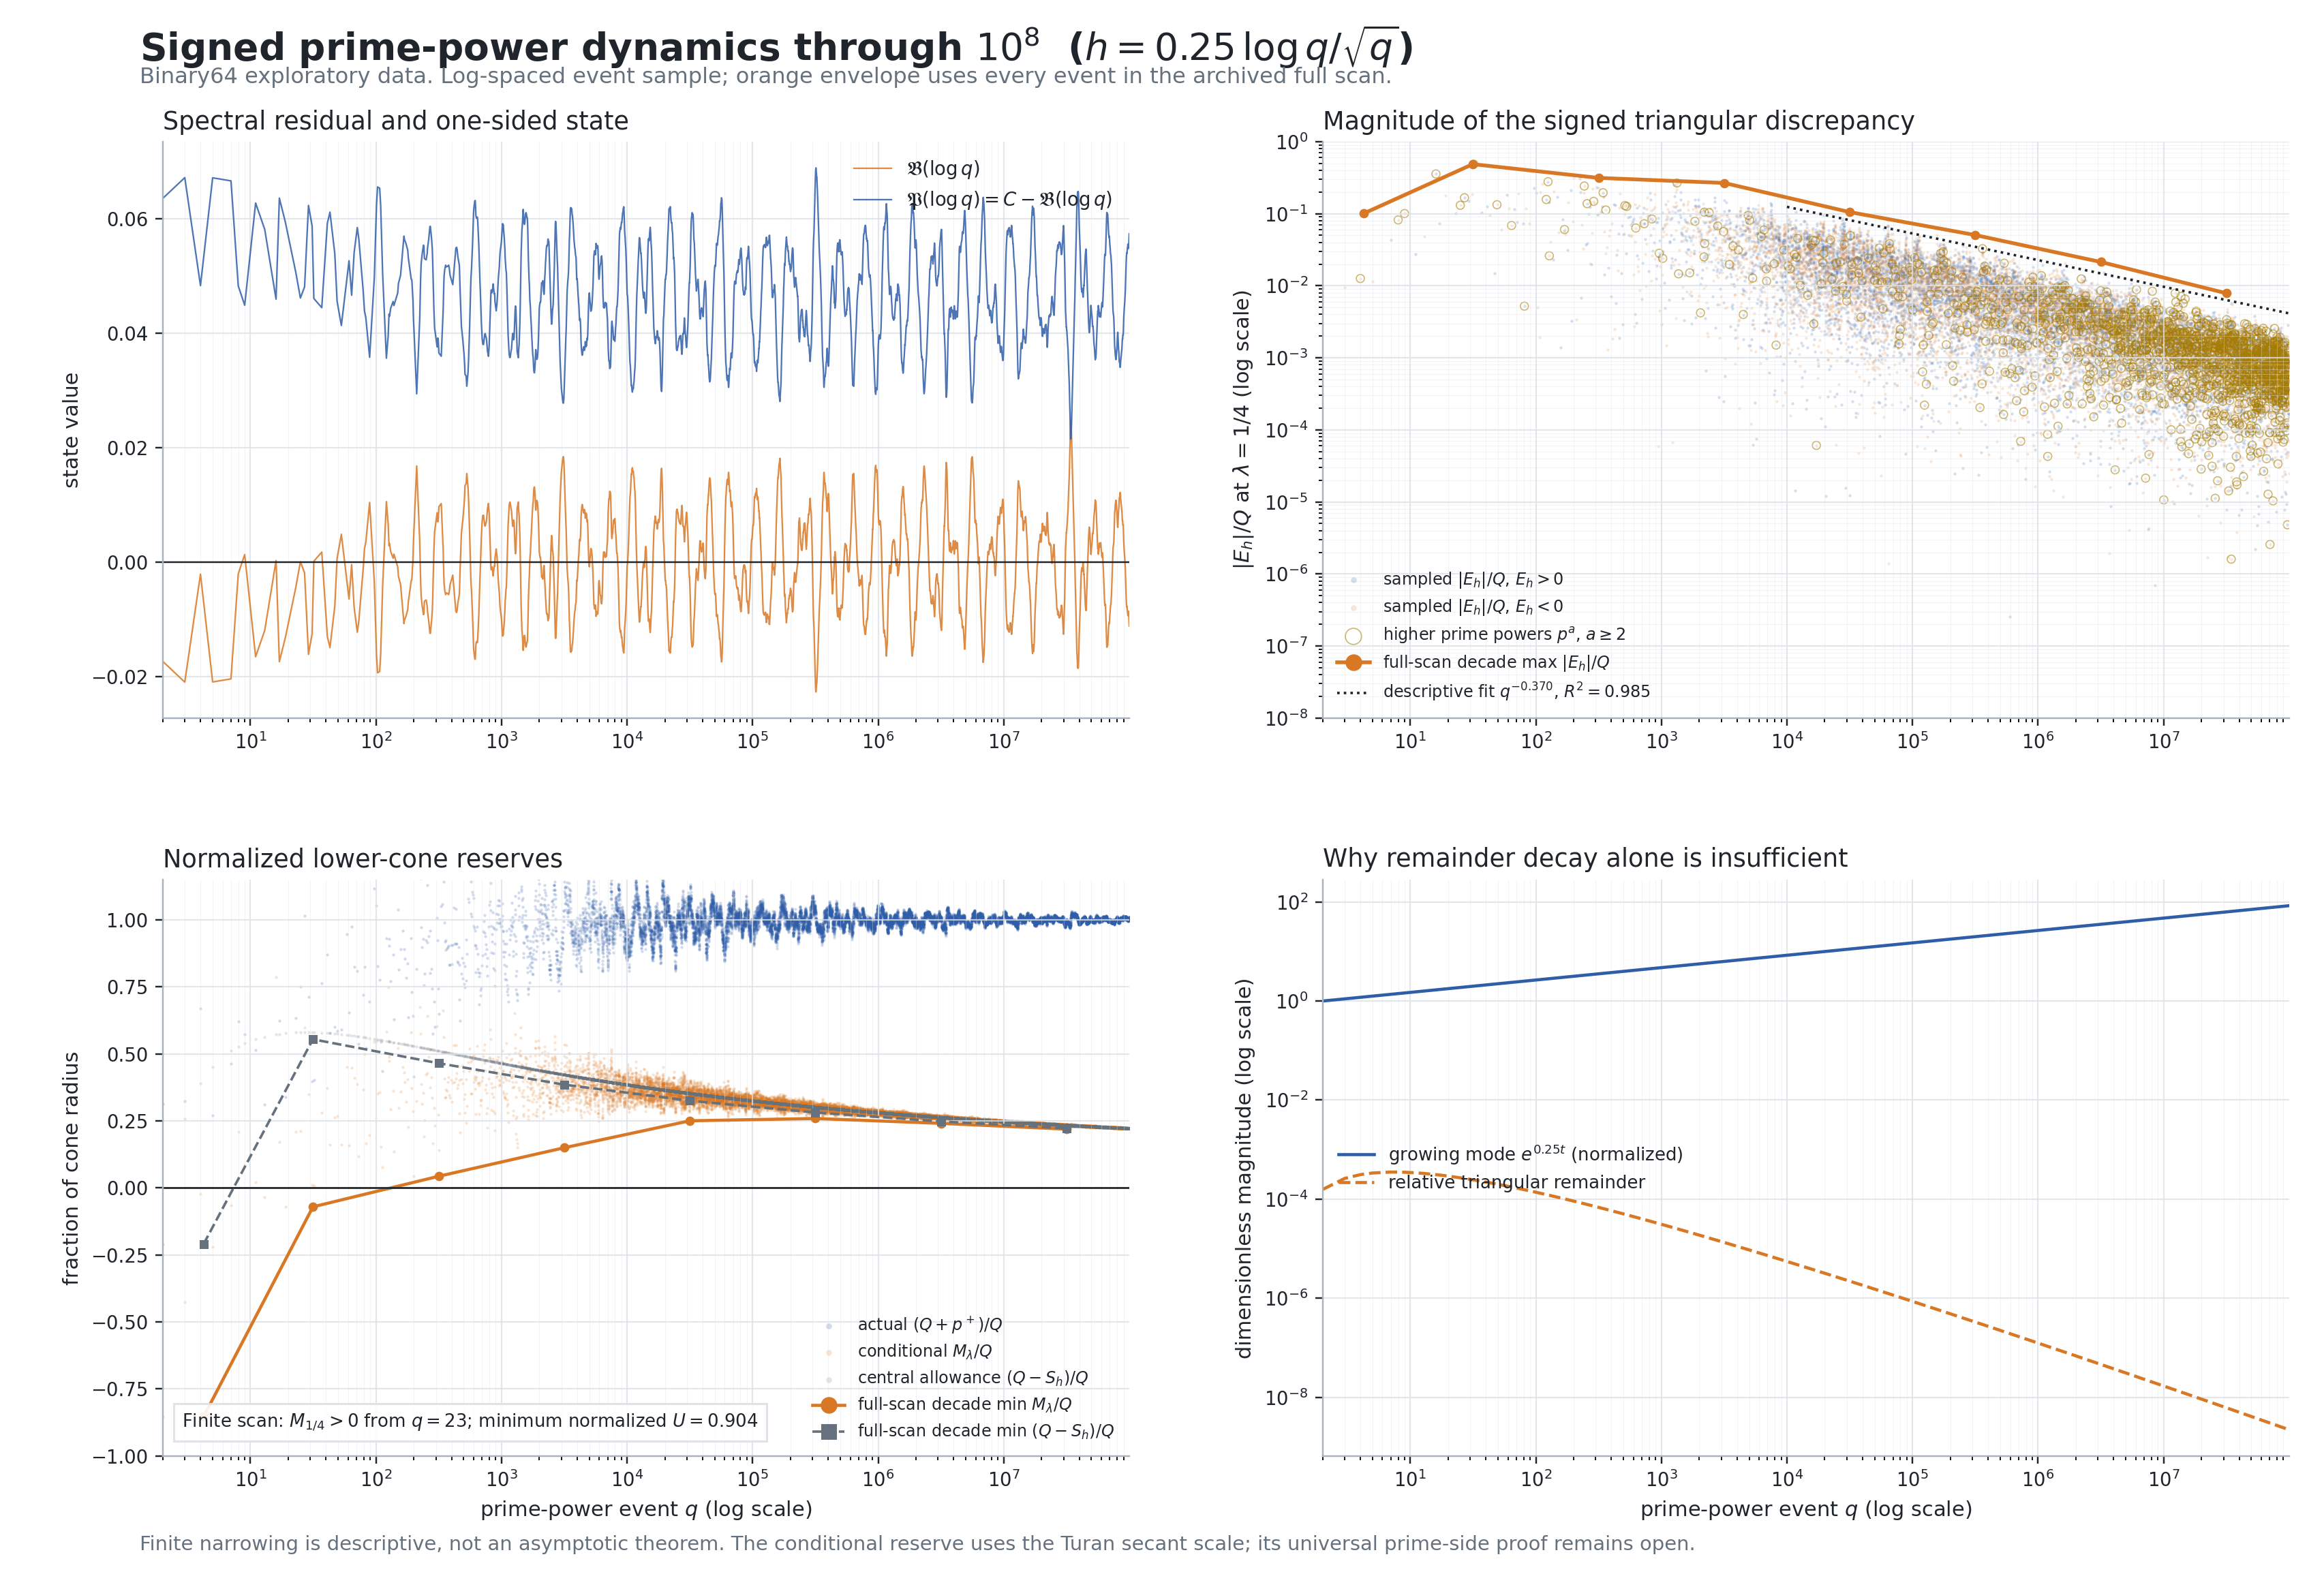
\includegraphics[width=0.84\linewidth]
  {figures/signed_triangular_dynamics_lambda_0p25.png}
\caption{Signed prime-power dynamics at \(\lambda=1/4\) through
\(q\le10^8\).  The upper panels show sampled states and the signed
triangular discrepancy, with orange maxima from the full scan.  The lower
panels compare normalized reserves and an analytic off-line test mode.  The
arithmetic panels are exploratory binary64 data, not interval certificates
or asymptotic theorems.}
\label{fig:signed-triangular-dynamics}
\end{figure}
\end{landscape}

Figure~\ref{fig:signed-triangular-dynamics} separates facts that must not be
conflated.  The upper-left panel displays a deterministic sample of
\(17\,836\) prime-power events: logarithmically spaced centers, every early
event through \(10^4\), and every higher prime power through \(10^8\).  The
curves are joined only to make the oscillatory shape visible.  The orange
envelope in the upper-right panel is stronger than the plotted sample: each
point is the maximum of \(|E_h|/Q\) over an entire decimal decade of the full
\(5\,762\,859\)-event scan.  Its fitted exponent \(-0.369607\) is descriptive
on this finite range only.

The lower-left panel compares the actual quantity needed after an event with
the modular RH-conditional lower bound.  Its finite positivity from the next
event \(q=23\), after the last failure at \(q=19\), is consistent with the
cone mechanism, but the interpretation of
\(M_{1/4}\) as a lower bound still requires \(U_{1/4}\ge0\).  The lower-right
panel is not arithmetic data.  It plots the exact analytic test
\(f_\mu(t)=e^{\mu t}\) with \(\mu=1/4\).  While
\(f_\mu(t)=q^{1/4}\) grows, \eqref{eq:exponential-relative-no-go} gives
\[
 \frac{|\mathcal T_\mu(t,h)|}{2h|f_\mu'(t)|}
 =\frac{\sinh(\mu h)}{\mu h}-1
 \sim\frac{\mu^2\lambda^2(\log q)^2}{6q}
 \longrightarrow0.
\]
Thus a shrinking relative triangular remainder measures local linearity on a
shrinking window; by itself it does not exclude a globally growing off-line
mode.  The infinite target remains the full combined condition
\eqref{eq:signed-triangular-cone-target}, or an unconditional proof of both
members of \eqref{eq:triangular-two-lemma-target}.

An implementation independent of the scanner reconstructed the prime-power
support and directly integrated the atomic and regular triangular terms.  At
\(q=997\), \(\lambda=1/2\), it obtained
\[
  \mathcal T^\triangle(t,h)=2hE_h
  =0.01298093486466930684879609372807777752292\ldots
\]
with an 80-digit residual of \(7.96\times10^{-79}\).  Ten tests passed with
\texttt{mpmath}~1.3.0: eight scanner regression tests and two independent
direct-QA tests.  One further regression test checks the two independent
binary64 evaluations of the exact hyperbolic decomposition, and four tests
check the scaling aggregation, archived maxima, source hashes, and plotted
sample count.  High-precision spot checks retained the signs of the reported
extremal values.  These tests check implementations and selected numerical
identities; they are not proofs of the exact algebra or of an asymptotic
law.  None of these calculations is an interval certificate, and finite
positivity of \(U_\lambda\) does not prove its RH-equivalent universal
extension.

\section{Executable certificates and reproducibility}

\subsection{Certificate summary}

\begin{center}
\begin{tabular}{p{0.42\textwidth}r}
\toprule
certificate & result\\
\midrule
ordinary-integer base & \(50\,400\) integers, no failure\\
support-\(11\) overlap & exact common endpoint \(55\,440\)\\
small CA bridge & \(503\) profiles, \(44\) ties, no failure\\
direct CA scan & \(3\,341\,978\) profiles, \(1\,427\) ties, no failure\\
finite \(D_*\) scan & \(3\,340\,551\) supports, no inconclusive case\\
extended residual cover & \(662\) segments, positive minimum\\
extended precision audit & \(4\,007\) matching intervals nested\\
all-integer cutoff audit & \(7\) matching intervals nested\\
\bottomrule
\end{tabular}
\end{center}

All paths below are relative to the root of the public software repository
\cite{polakrepo2026}.  The complete companion directory is
\url{https://github.com/robopol/Riemann-hypothesis/tree/main/verification/finite_robin_prime_power}.
The canonical certifiers and reports are:

\begingroup
\small
\begin{longtable}{p{0.25\textwidth}p{0.68\textwidth}}
\toprule
purpose & artifact and SHA-256\\
\midrule
\endhead

direct all-profile scan &
\path{verification/finite_robin_prime_power/test_ca_all_profile_interval_certificate.py}\\
&
\sha{8da8ad3d63b6dec8}{ffd4838b968a0add}{ed4c26eb5810fa29}{69dadb917f691077}\\
&
\path{verification/finite_robin_prime_power/ca_all_profile_interval_certificate_report.json}\\
&
\sha{8ac1ee276df64cc9}{1d93b483b501d34f}{8a9b69408d2fb065}{0d4bab8f43304f83}\\
\addlinespace

finite \(D_*\) sweep &
\path{verification/finite_robin_prime_power/test_ca_exact_buffer_interval_certifier.py}\\
&
\sha{add8f04a2e02b606}{491c1bdf6aab4fcb}{23f5d10e2db20232}{6fded0c5035d5ef2}\\
&
\path{verification/finite_robin_prime_power/ca_exact_buffer_interval_certificate_report.json}\\
&
\sha{57c14d33aa47b7dd}{ff012043304151fc}{9b11b50a114c2634}{665f7455ce80dba1}\\
\addlinespace

analytic \(D_*\) continuation &
\path{verification/finite_robin_prime_power/test_asymptotic_dstar_lower_bound.py}\\
&
\sha{c7981a2fdec34211}{e07434d82931c2ac}{534a20e384fdace3}{1b4ee6d79a8211b5}\\
&
\path{verification/finite_robin_prime_power/asymptotic_dstar_lower_bound_report.json}\\
&
\sha{ea33332d7acade20}{b35409131a6a5aca}{c00d722cf3439d9b}{36cb7992d296fa18}\\
\addlinespace

extended residual &
\path{verification/finite_robin_prime_power/test_ca_residual_upward_extended_certificate.py}\\
&
\sha{165f7a069c93ede7}{9709ed559fdd1a99}{08e41230fd4b5208}{44931789a97d3e95}\\
&
\path{verification/finite_robin_prime_power/ca_residual_upward_extended_certificate_report.json}\\
&
\sha{938713a1e1443196}{e349269d9f88f429}{d3859aa262fbf110}{42733c6ef1278263}\\
&
\path{verification/finite_robin_prime_power/ca_residual_upward_extended_certificate_p80_report.json}\\
&
\sha{41244347c6366c33}{21dc653235b9db32}{008e38678654d2f8}{99838b7f5c2ee8a1}\\
\addlinespace

integer base &
\path{verification/finite_robin_prime_power/test_robin_base_5041_55440_interval.py}\\
&
\sha{ee296aa4a9e57e57}{6da69a114e5983d9}{dad172d89e35d149}{8c83a1cff211c1aa}\\
&
\path{verification/finite_robin_prime_power/robin_base_5041_55440_interval_report.json}\\
&
\sha{161381cb69f55030}{f2f6bb0c57c65183}{83aa66a7d65165cf}{98e1686aa013cf45}\\
\addlinespace

support-\(11\) overlap &
\path{verification/finite_robin_prime_power/test_ca_support_11_overlap_certificate.py}\\
&
\sha{660420eba61fa0ad}{61df16ed6117dfd7}{6ac84adb78cff289}{2c44e0b500de29a9}\\
&
\path{verification/finite_robin_prime_power/ca_support_11_overlap_certificate_report.json}\\
&
\sha{af903d574499c2b9}{450b9afed9b4799d}{3d01a668eb300973}{06d61ba97da1a0bd}\\
\addlinespace

small CA bridge &
\path{verification/finite_robin_prime_power/test_ca_all_profile_interval_certificate.py}\\
&
\sha{8da8ad3d63b6dec8}{ffd4838b968a0add}{ed4c26eb5810fa29}{69dadb917f691077}\\
&
\path{verification/finite_robin_prime_power/ca_all_profile_bridge_11_3299_report.json}\\
&
\sha{e29d66dde12af0e7}{73d86827b0237ed3}{23f62abfd19bc7fe}{028a7e065782e5ca}\\
\addlinespace

all-integer cutoff &
\path{verification/finite_robin_prime_power/test_ca_all_integer_cutoff_certificate.py}\\
&
\sha{df1238bee0184a3d}{ccebdcaf72920b93}{62984ec845273692}{a786bf69030e4052}\\
&
\path{verification/finite_robin_prime_power/ca_all_integer_cutoff_certificate_report.json}\\
&
\sha{0ba63f2645fc5c31}{2aa00890daff8b87}{b720e68656c5cddf}{c31dd1465284f8f3}\\
&
\path{verification/finite_robin_prime_power/ca_all_integer_cutoff_certificate_p80_report.json}\\
&
\sha{5dde972048d365ef}{e11a9305bec698a0}{f0c56de0e27957f8}{d72f67a72b00351e}\\
\addlinespace

paper manifest and precision audit &
\path{verification/finite_robin_prime_power/test_finite_robin_paper_manifest.py}\\
&
\sha{4feeafbe0178e482}{5191b0244b280a14}{447d21f9792e0282}{a2204a8910d0617a}\\
\bottomrule
\end{longtable}
\endgroup

\subsection{Exploratory signed-dynamics artifacts}

The following artifacts support only the binary64 diagnostics and independent
numerical QA in Section~\ref{sec:signed-dynamics}.  They are deliberately
separated from the directed-interval certificates above.

\begingroup
\small
\begin{longtable}{p{0.25\textwidth}p{0.68\textwidth}}
\toprule
purpose & artifact and SHA-256\\
\midrule
\endhead

event-driven implementation &
\path{verification/finite_robin_prime_power/exploratory_b_cell_dynamics.py}\\
&
\sha{1f1722248765f2ba}{314fbb5c17cd7727}{a58ef363f00254ed}{9ff9edb0fbd68c21}\\
\addlinespace

full finite scan report &
\path{verification/finite_robin_prime_power/exploratory_b_cell_dynamics_report.json}\\
&
\sha{5c610b2e08ccc94b}{30b158d1cd578daf}{ad3189042491aa4e}{6d7006670c25da41}\\
\addlinespace

moderate-range regression test &
\path{verification/finite_robin_prime_power/test_exploratory_b_cell_dynamics.py}\\
&
\sha{446f0e22fe617c1e}{d7809dd3d2e78f1a}{10420cd611be4c8b}{33239ceb5e17b773}\\
\addlinespace

derivation and experiment log &
\path{verification/finite_robin_prime_power/B_Prime_Power_Cell_Dynamics_Investigation_2026-08-04.md}\\
&
\sha{acb81a8c38101b3e}{5fada926faf75ac2}{4a05e67d7d231566}{7c6aac49bff22b8b}\\
\addlinespace

signed-triangular scanner &
\path{verification/finite_robin_prime_power/exploratory_signed_triangular_scan.py}\\
&
\sha{d03e166a4bd5fde6}{a9ed8ed583ab74df}{31db7d0fc214090b}{d1fb9160519b9daa}\\
\addlinespace

eventwise prime-side helper &
\path{verification/finite_robin_prime_power/exploratory_eventwise_reserve_scan.py}\\
&
\sha{75f4889ae5133f25}{71e05233394197fb}{09545f5d5d0ebc75}{163707521bc5e77b}\\
\addlinespace

signed-triangular \(10^8\) report &
\path{verification/finite_robin_prime_power/exploratory_signed_triangular_scan_1e8_report.json}\\
&
\sha{b464e154ee46a8ca}{f9a223dda8c60ebc}{acd17eefa4d9548c}{33b10e16232743a4}\\
\addlinespace

signed-triangular regression test &
\path{verification/finite_robin_prime_power/test_exploratory_signed_triangular_scan.py}\\
&
\sha{ab61a564273346f8}{38af4d13498b02fb}{3f2e01d078f2b32f}{030fe86d6d1672f7}\\
\addlinespace

independent triangular direct QA &
\path{verification/finite_robin_prime_power/test_exploratory_signed_triangular_direct_qa.py}\\
&
\sha{b53b528e32d09f27}{ad1d9f35dbae9800}{d0f665ce508eaaba}{cc7d119e96fdae92}\\
\addlinespace

exact \(E_h\) investigation &
\path{verification/finite_robin_prime_power/Eh_Decay_Analytic_Investigation_2026-08-05.md}\\
&
\sha{de47320a9142d014}{2f6dbdfdab60e6ea}{e6c1a935f923530a}{69c39d4166fee4c1}\\
\addlinespace

prime-side derivation &
\path{verification/finite_robin_prime_power/Prime_Side_Eh_Decay_Derivation_2026-08-05.md}\\
&
\sha{2a05e34cef9ae3b0}{b5693e70b0da6eb2}{f33d118cd56385bd}{b6708616fe1b38b8}\\
\addlinespace

exact-decomposition regression test &
\path{verification/finite_robin_prime_power/test_prime_side_eh_decomposition.py}\\
&
\sha{6ba6b5e18067cc24}{16df8624341a29d4}{c5b4d47910ce1f5e}{21c264186d4837bd}\\
\addlinespace

full-population scaling audit &
\path{verification/finite_robin_prime_power/audit_eh_scaling_law.py}\\
&
\sha{f8c3d03963705cdd}{ead22ab07ff67a8f}{8d17855ee2d363cb}{8d0f5d0eebe6100b}\\
\addlinespace

scaling-audit report &
\path{verification/finite_robin_prime_power/eh_scaling_law_audit_report.json}\\
&
\sha{0aaf4eb5dd456e94}{417853dcf4609d43}{c0113fb5b14a0979}{28589e9f56d3fa4b}\\
\addlinespace

scaling-audit regression test &
\path{verification/finite_robin_prime_power/test_audit_eh_scaling_law.py}\\
&
\sha{f2987d0407dd59af}{4d0606d12f617ba5}{0ff7e0afb9f587d7}{8c12116226e35d6d}\\
\addlinespace

scaling-audit analysis &
\path{verification/finite_robin_prime_power/Eh_Scaling_Law_Audit_2026-08-05.md}\\
&
\sha{11132a22a95e0937}{fc323739b3ef63e9}{4febb9455e14f1e9}{4d616b8f9fec77a8}\\
\addlinespace

spectral and almost-all analysis &
\path{verification/finite_robin_prime_power/Spectral_Eh_Decay_Analysis_2026-08-05.md}\\
&
\sha{35c2f9a73b21969a}{f7c9e893e7dc2f54}{170926b74aaff63b}{ba0de165770f5870}\\
\addlinespace

signed-dynamics figure generator &
\path{verification/finite_robin_prime_power/plot_signed_triangular_dynamics.py}\\
&
\sha{2ede87d1f57dea11}{3ad9d24ee396c527}{86c3261b5357c3b1}{c29e03ff975b9237}\\
\addlinespace

paper figure, raster &
\path{papers/figures/signed_triangular_dynamics_lambda_0p25.png}\\
&
\sha{3bcbf276c578c61f}{ed17548ac6608141}{4caa9238fff8dcec}{78e9c37623cdb48a}\\
\addlinespace

paper figure, vector &
\path{papers/figures/signed_triangular_dynamics_lambda_0p25.svg}\\
&
\sha{114f1fd10ccc8338}{d90bbdce8e85e013}{8ae0ffaf3517a562}{91422e19113b092b}\\
\addlinespace

plotted deterministic sample &
\path{papers/figures/signed_triangular_dynamics_lambda_0p25_sample.csv}\\
&
\sha{e35fd4e97c829f53}{10bdba29d5d668a8}{3f9bcb7b1d7ed40e}{9a2c695b9bd218bb}\\
\bottomrule
\end{longtable}
\endgroup

The common prime-stream SHA-256 through \(\Xdirect\) is
\begin{center}
  \sha{9438df02de33467c}{1ed4307c0a801c2c}{57777e00bb7413b1}{7ce955a117c8b2c9}.
\end{center}
The top-level cutoff certifier reopens the canonical dependency reports,
checks their domains and PASS fields, and verifies all direct plus six
transitive source/report hashes against the current files.

\subsection{Integrity audit and recomputation}

\begin{verbatim}
Set-Location verification/finite_robin_prime_power

python test_finite_robin_paper_manifest.py
python test_exploratory_b_cell_dynamics.py
python test_exploratory_signed_triangular_scan.py
python test_exploratory_signed_triangular_direct_qa.py
python test_prime_side_eh_decomposition.py
python test_audit_eh_scaling_law.py
\end{verbatim}

The first command is the canonical non-destructive audit of the archived
release: it reopens the reports, verifies their listed hashes and headline
values, and checks all (4,007+7) cross-precision interval inclusions.  The
second command is a moderate-range regression test of the exploratory
prime-power implementation.  The next two commands test the signed
triangular scanner and its independent direct reconstruction; the 80-digit
branch requires \texttt{mpmath}.  The final two commands check the exact
hyperbolic decomposition through independent evaluation paths and validate
the saved full-population scaling aggregation without repeating the
\(10^8\) scan.

Exact parameters for fresh recomputation, including the full direct sweep,
the binary64 cell scan through \(\Xdirect\), the signed-triangular scan
through \(10^8\), and deterministic reproduction of
Figure~\ref{fig:signed-triangular-dynamics}, are recorded in
\path{verification/finite_robin_prime_power/README.md}.  Fresh runs must write
to alternate report names or be made in a disposable copy.  The archived JSON
files deliberately record environment-dependent metadata such as absolute
paths, command-line arguments, and timings, so a newly generated report is
expected to have a different whole-file SHA-256 even when its certified
mathematical fields agree.  A release intended for external verification
should archive the complete repository under an immutable commit and a
persistent DOI; branch-relative paths alone are not a permanent citation.

\subsection{Directed arithmetic and trusted base}

The interval implementations use separate floor and ceiling decimal contexts
for arithmetic operations.  Logarithms and square roots are evaluated at
higher precision and padded outward by explicit ulps.  Euler's constant is
self-enclosed by harmonic-number inequalities, and \(\pi\) is self-enclosed
by Machin's formula where required.  Integer divisor sums, prime powers,
threshold indices, and sieve state use exact Python integers.

The trusted base consists of:
\begin{itemize}
  \item the analytic lemmas stated in this paper;
  \item the cited published theorems;
  \item CPython integer and Decimal semantics in the recorded environment;
  \item correctness of the deterministic sieve and certificate programs;
  \item correctness of the operating system and hardware execution.
\end{itemize}
Independent \(60\)- and \(80\)-digit runs give nested enclosures.  This
substantially exceeds ordinary floating-point evidence, but it is not a
formal verification of the implementation.

\section{Present barrier and rigor boundary}

The same-point scalar envelope used in the upper certificate is positive at
\[
  1.64967\times10^{23}
\]
by at least \(3.2833942493\times10^{-7}\), but is negative at
\[
  1.64968\times10^{23}
\]
by more than \(1.5193588576\times10^{-6}\).  Nothing singular happens to a CA
profile at this decimal endpoint.  The sign change belongs only to the
absolute lower envelope.

For fixed verified height \(T\), the dominant term in
\eqref{eq:high-zero-loss} grows essentially as
\[
  S_2(T)\sqrt{x}.
\]
In contrast, the explicit lower reserve \(D_{\mathrm{lb}}(x)\) approaches a
finite constant.  Therefore the present absolute high-zero treatment must
eventually exhaust the deterministic reserve.

There are now two distinct continuation routes.  To extend the
\emph{finite certificate}, one may raise the rigorous zero-verification
height, sharpen the directed high-zero or off-line-zero estimates, or change
the smoothing kernel.  To address the \emph{universal quantifier}, the signed
formulation in Section~\ref{sec:signed-dynamics} gives a more concrete target:
prove the eventwise reserve inequality
\eqref{eq:universal-kick-target}; equivalently, prove the sharp combined
signed-window inequality \eqref{eq:signed-triangular-cone-target}.  A stronger
modular route is the pair \eqref{eq:triangular-two-lemma-target}, and a fourth
possibility is a block estimate controlling the signed cross-work in
\eqref{eq:polynomial-energy-kick}.  The Tur\'an member of the modular pair is
itself RH-strength and is presently available here only under RH.  Thus a
tighter absolute envelope is not the only structural route, although it
remains the mechanism behind the finite theorem proved here.

The prime-side reduction \eqref{eq:additive-E-reduction} identifies the raw
numerator with an odd triangular von Mangoldt discrepancy up to an explicit
smaller term.  Proposition~\ref{prop:almost-all-E-decay} controls that
numerator in mean square for continuous centers, but a Lebesgue almost-all
theorem cannot select the prescribed measure-zero sequence \(q=p^a\), and it
does not control the ratio to \(Q\).  The final signed step therefore remains
a uniform one-sided or two-sided short-interval estimate at every
prime-power center, coupled to the central-secant reserve rather than
detached from it.

The following points delimit the claim.
\begin{enumerate}
  \item No full-RH assumption is made.  The Platt--Trudgian result is a
        published finite-height theorem.
  \item This paper does not use a universal assertion
        \(\theta(p)<p\).  The primary layer bound uses the global
        Rosser--Schoenfeld estimate; an optional stronger layer audit uses
        B\"uthe only in its stated finite range.  The support-to-size
        conversion uses the lower Dusart estimate
        \eqref{eq:dusart-theta}.
  \item The negative scalar envelope above the endpoint is not a
        counterexample to Robin's inequality.
  \item The signed buffer identity, cell equation, cone criterion, exact
        triangular transfer, and prime-side reduction are unconditional.
        The Tur\'an secant bound in
        Proposition~\ref{prop:conditional-turan} explicitly assumes RH and is
        not used in either finite theorem.
  \item The binary64 scans through \(\Xdirect\) and \(10^8\) are exploratory.
        The unconditional mean-square theorem proves decay in measure only
        for the raw continuous-center numerator.  Neither it nor the scans
        establish a universal kick criterion, a universal Tur\'an defect,
        eventwise decay at \(q=p^a\), or an asymptotic bound for \(E_h/Q\).
  \item The result proves nothing for integers above
        \(10^{7.1\times10^{22}}\), and it does not prove the Riemann
        hypothesis.
\end{enumerate}

\section{Conclusion}

The full-support CA ledger admits the exact prime-power reduction
\[
  \Ggap(n)
  =
  \Rinf(x)+\Btwo(n,x)
  +R_{\mathrm{core}}(n,x)-\Cpi(x),
\]
with a strictly positive, profile-independent deterministic buffer \(D_*(x)\).
An exhaustive CA profile computation closes the lower finite support range,
while a directed analytic residual certificate continues the result to
\(1.64967\times10^{23}\).  Robin's consecutive-CA convexity proposition and
an explicit support-to-size estimate then give the all-integer cutoff
\[
  5041\le n\le10^{7.1\times10^{22}}.
\]
The remaining obstruction is not the finite prime-power reduction or the CA
handoff.  For the present finite certificate it is the absolute treatment of
the unverified high-zero tail beyond the endpoint.  At the signed level, the
same obstruction has been reduced to an exact hybrid system: smooth cells
replenish the cone reserve \(M_B\), and each prime power \(q\) withdraws
exactly \(\Lambda(q)/\sqrt q\).  The initial cone is elementary, and the
remaining universal target is the prime-power inequality
\eqref{eq:universal-kick-target}.  The signed triangular identity rewrites
that same lower-cone transfer as the sharp short-window inequality
\eqref{eq:signed-triangular-cone-target} on the natural additive scale
\(\sqrt q\log q\).  The exact hyperbolic decomposition and its additive
corollary further isolate the arithmetic numerator as
\[
 E_h(q)=\frac{\Delta_H(q)}{2\sqrt q}
 +O_\lambda\!\left(\frac{(\log q)^3}{\sqrt q}\right).
\]
The full scan shows an approximately stationary bulk after normalization by
\(Q\log q/\sqrt q\), and the Selberg-integral argument proves unconditional
decay in measure for the corresponding raw discrepancy at continuous
centers.  Neither statement is uniform on the prime-power event set or
controls a small denominator \(Q\).  RH conditionally supplies a Tur\'an
secant bound whose
critical window is \(h=(\log q)/(4\sqrt q)\), including a favorable
next-order correction.  The scan through \(10^8\) finds no negative Tur\'an
defect and finds a positive conditional reserve after a small finite base,
but it is ordinary floating-point evidence only.  Moreover, the exponential
mode calculation \eqref{eq:exponential-triangular-no-go} proves that decay of
the triangular discrepancy alone cannot exclude an off-line mode.  What
remains is an unconditional prime-side proof of the combined inequality, the
two-lemma target, or an adequate block signed-work estimate.  None is proved
here, so the conclusion remains a finite verification rather than a proof of
RH.

\begin{thebibliography}{99}

\bibitem{robin1984}
G.~Robin,
\newblock Grandes valeurs de la fonction somme des diviseurs et hypothese de
Riemann,
\newblock \emph{J. Math. Pures Appl. (9)} 63 (1984), 187--213,
\newblock MR0774171.

\bibitem{alaogluerdos1944}
L.~Alaoglu and P.~Erd\H{o}s,
\newblock On highly composite and similar numbers,
\newblock \emph{Trans. Amer. Math. Soc.} 56 (1944), 448--469,
\newblock doi:
\href{https://doi.org/10.1090/S0002-9947-1944-0011087-2}
{10.1090/S0002-9947-1944-0011087-2}.

\bibitem{dusartprime1999}
P.~Dusart,
\newblock The \(k\)-th prime is greater than
\(k(\log k+\log\log k-1)\) for \(k\ge2\),
\newblock \emph{Math. Comp.} 68 (1999), 411--415,
\newblock doi:
\href{https://doi.org/10.1090/S0025-5718-99-01037-6}
{10.1090/S0025-5718-99-01037-6}.

\bibitem{dusarttheta1999}
P.~Dusart,
\newblock In\'egalit\'es explicites pour \(\psi(x)\), \(\theta(x)\),
\(\pi(x)\) et les nombres premiers,
\newblock \emph{C. R. Math. Rep. Acad. Sci. Canada} 21 (1999), 53--59,
\newblock \url{https://mathreports.ca/article/inegalites-explicites-pour%F0%9D%9C%93x%F0%9D%9C%83x%F0%9D%9C%8Bx-et-les-nombres-premier/}.

\bibitem{rosserschoenfeld1962}
J.~B.~Rosser and L.~Schoenfeld,
\newblock Approximate formulas for some functions of prime numbers,
\newblock \emph{Illinois J. Math.} 6 (1962), 64--94,
\newblock doi:
\href{https://doi.org/10.1215/ijm/1255631807}
{10.1215/ijm/1255631807}.

\bibitem{buthe2016}
J.~B\"uthe,
\newblock Estimating \(\pi(x)\) and related functions under partial RH
assumptions,
\newblock \emph{Math. Comp.} 85 (2016), 2483--2498,
\newblock doi:
\href{https://doi.org/10.1090/mcom/3060}{10.1090/mcom/3060}.

\bibitem{buthe2018}
J.~B\"uthe,
\newblock An analytic method for bounding \(\psi(x)\),
\newblock \emph{Math. Comp.} 87 (2018), 1991--2009,
\newblock doi:
\href{https://doi.org/10.1090/mcom/3264}{10.1090/mcom/3264}.

\bibitem{platttrudgian2021}
D.~Platt and T.~Trudgian,
\newblock The Riemann hypothesis is true up to \(3\cdot10^{12}\),
\newblock \emph{Bull. Lond. Math. Soc.} 53 (2021), 792--797,
\newblock doi:
\href{https://doi.org/10.1112/blms.12460}{10.1112/blms.12460}.

\bibitem{hsw2022}
E.~Hasanalizade, Q.~Shen and P.-J.~Wong,
\newblock Counting zeros of the Riemann zeta function,
\newblock \emph{J. Number Theory} 235 (2022), 219--241,
\newblock doi:
\href{https://doi.org/10.1016/j.jnt.2021.06.032}
{10.1016/j.jnt.2021.06.032}.

\bibitem{titchmarsh1986}
E.~C.~Titchmarsh,
\newblock \emph{The Theory of the Riemann Zeta-Function},
\newblock 2nd ed., revised by D.~R.~Heath-Brown,
\newblock Oxford University Press, 1986.

\bibitem{weil1952}
A.~Weil,
\newblock Sur les formules explicites de la th\'eorie des nombres premiers,
\newblock \emph{Comm. S\'em. Math. Univ. Lund
[Medd. Lunds Univ. Mat. Sem.]}, Tome Suppl\'ementaire (1952), 252--265.

\bibitem{SaffariVaughan1977}
B.~Saffari and R.~C.~Vaughan,
\newblock On the fractional parts of \(x/n\) and related sequences. II,
\newblock \emph{Ann. Inst. Fourier (Grenoble)} 27 (1977), no.~2, 1--30,
\newblock doi:
\href{https://doi.org/10.5802/aif.649}{10.5802/aif.649}.

\bibitem{MontgomerySound2004}
H.~L.~Montgomery and K.~Soundararajan,
\newblock Primes in short intervals,
\newblock \emph{Comm. Math. Phys.} 252 (2004), 589--617,
\newblock doi:
\href{https://doi.org/10.1007/s00220-004-1222-4}
{10.1007/s00220-004-1222-4}.

\bibitem{Chan2003}
T.~H.~Chan,
\newblock More precise pair correlation of zeros and primes in short
intervals,
\newblock \emph{J. London Math. Soc. (2)} 68 (2003), 579--598,
\newblock doi:
\href{https://doi.org/10.1112/S0024610703004769}
{10.1112/S0024610703004769}.

\bibitem{FordSoundZah2009}
K.~Ford, K.~Soundararajan and A.~Zaharescu,
\newblock On the distribution of imaginary parts of zeros of the Riemann
zeta function, II,
\newblock \emph{Math. Ann.} 343 (2009), 487--505,
\newblock \url{https://arxiv.org/abs/0805.2745}.

\bibitem{GuthMaynard2026}
L.~Guth and J.~Maynard,
\newblock New large value estimates for Dirichlet polynomials,
\newblock \emph{Ann. of Math. (2)} 203 (2026), 623--675,
\newblock doi:
\href{https://doi.org/10.4007/annals.2026.203.2.6}
{10.4007/annals.2026.203.2.6}.

\bibitem{CullyHugillDudek2022}
M.~Cully-Hugill and A.~W.~Dudek,
\newblock A conditional explicit result for the prime number theorem in
short intervals,
\newblock arXiv:1902.05065v2, 2022,
\newblock \url{https://arxiv.org/abs/1902.05065}.

\bibitem{Suzuki2023}
M.~Suzuki,
\newblock Aspects of the screw function corresponding to the Riemann
zeta-function,
\newblock \emph{J. London Math. Soc.} 108 (2023), 1448--1487,
\newblock doi:
\href{https://doi.org/10.1112/jlms.12785}{10.1112/jlms.12785}.

\bibitem{widder1941}
D.~V.~Widder,
\newblock \emph{The Laplace Transform},
\newblock Princeton Mathematical Series, vol.~6,
\newblock Princeton University Press, 1941.

\bibitem{polakstatus2026}
R.~Polak,
\newblock Corrected status of the Robin--MVDC programme,
\newblock companion manuscript, 2026.

\bibitem{polakrepo2026}
R.~Polak,
\newblock Riemann-hypothesis: computational certificates and support data,
\newblock software repository, 2026,
\newblock \url{https://github.com/robopol/Riemann-hypothesis}.

\end{thebibliography}

\end{document}
